\documentclass[9pt,a4paper]{extarticle}
\usepackage[a4paper,top=20mm,bottom=20mm,left=15mm,right=15mm,columnsep=6mm,headsep=5mm]{geometry}
\usepackage{fontspec}
\setmainfont{TeX Gyre Termes}
\setsansfont{TeX Gyre Heros}
\setmonofont{DejaVu Sans Mono}[Scale=0.85]
\usepackage{amsmath,amssymb}
\usepackage{graphicx,xcolor,booktabs,tabularx,array,enumitem,fancyhdr,titlesec,caption,microtype}
\usepackage{newunicodechar}
\usepackage[hidelinks]{hyperref}
\usepackage{url}
\urlstyle{same}
\definecolor{elsblue}{HTML}{1F5FA6}
\definecolor{rulegray}{HTML}{9A9A9A}
\definecolor{bandgray}{HTML}{F1F1F1}
\newfontfamily\fallback{DejaVu Serif}[Scale=0.92]
\newunicodechar{−}{\ensuremath{-}}
\newunicodechar{≥}{\ensuremath{\geq}}
\newunicodechar{≤}{\ensuremath{\leq}}
\newunicodechar{∩}{\ensuremath{\cap}}
\newunicodechar{∈}{\ensuremath{\in}}
\newunicodechar{Δ}{\ensuremath{\Delta}}
\newunicodechar{×}{\ensuremath{\times}}
\newunicodechar{α}{\ensuremath{\alpha}}
\newunicodechar{′}{\ensuremath{'}}
\newunicodechar{→}{\ensuremath{\rightarrow}}
\newunicodechar{⇒}{\ensuremath{\Rightarrow}}
\newunicodechar{≈}{\ensuremath{\approx}}
\newunicodechar{²}{\textsuperscript{2}}
\newcommand{\seclabel}[1]{{\fontsize{8}{10}\selectfont\addfontfeatures{LetterSpace=25}\MakeUppercase{#1}}\par\vspace{1pt}{\color{rulegray}\hrule height 0.4pt}\vspace{3pt}}
\newcommand{\tabcap}[2]{{\footnotesize\textbf{Bảng #1}\par\vspace{1pt}#2\par}\vspace{3pt}\scriptsize}
\newcommand{\tabnote}[1]{\par\vspace{2pt}{\scriptsize\raggedright #1\par}}
\newcommand{\figcap}[2]{\par\vspace{3pt}{\footnotesize\raggedright\textbf{Hình #1.} #2\par}}
\providecommand{\tightlist}{\setlength{\itemsep}{0pt}\setlength{\parskip}{0pt}}
\setcounter{secnumdepth}{-1}
\titleformat{\section}{\normalsize\bfseries}{}{0pt}{}
\titlespacing*{\section}{0pt}{9pt}{4pt}
\titleformat{\subsection}{\normalsize\itshape}{}{0pt}{}
\titlespacing*{\subsection}{0pt}{7pt}{3pt}
\titleformat{\subsubsection}{\small\bfseries}{}{0pt}{}
\setlength{\parindent}{1em}
\setlength{\parskip}{0pt}\setlength{\emergencystretch}{3em}
\setlist{leftmargin=1.4em,itemsep=1pt,topsep=2pt}
\pagestyle{fancy}\fancyhf{}
\fancyhead[L]{\footnotesize C.-D. Tran}
\fancyhead[R]{\footnotesize Bản thảo PLCA-Hypertension (tiếng Việt)}
\fancyfoot[C]{\footnotesize\thepage}
\renewcommand{\headrulewidth}{0pt}
\fancypagestyle{first}{\fancyhf{}\fancyfoot[C]{\footnotesize\thepage}\renewcommand{\headrulewidth}{0pt}}
\setlength{\abovecaptionskip}{2pt}
\renewcommand{\arraystretch}{1.15}
\setlength{\tabcolsep}{3.5pt}
\newcounter{refc}
\begin{document}
\thispagestyle{first}

\twocolumn[{%
\begin{center}
{\small\color{elsblue} PLCA-Hypertension \textperiodcentered{} Bản thảo tiếng Việt để review \textperiodcentered{} chưa qua bình duyệt}\\[2pt]
{\color{rulegray}\rule{\textwidth}{0.4pt}}\\[-1pt]
\colorbox{bandgray}{\parbox{\dimexpr\textwidth-2\fboxsep}{\centering\vspace{5pt}
{\fontsize{17}{20}\selectfont\color{black!85} Bản thảo dự kiến nộp \textit{International Journal of Medical Informatics}}\\[3pt]
{\small\color{elsblue} Dàn trang mô phỏng bố cục bài báo, dùng để đọc và góp ý}\vspace{5pt}}}\\[-1pt]
{\color{elsblue}\rule{\textwidth}{1.6pt}}
\end{center}
\vspace{6pt}
{\raggedright\fontsize{17}{21}\selectfont Attribution is not mitigation: A paired-label counterfactual audit of hypertension classification models\par}
\vspace{4pt}
{\raggedright\large\itshape\color{black!75} Đóng góp không đồng nghĩa với khắc phục: kiểm định giải thích phản thực tế bằng nhãn kép cho các mô hình phân loại tăng huyết áp\par}
\vspace{8pt}
{\large Cong-Danh Tran\textsuperscript{\,a}}\\[3pt]
{\footnotesize\itshape \textsuperscript{a}\,[Đơn vị, Thành phố, Việt Nam]}
\vspace{10pt}

\seclabel{ĐIỂM NỔI BẬT}
\vspace{-2pt}
{\small\begin{itemize}[leftmargin=10pt,itemsep=0pt,topsep=2pt,label=\textbullet]
\item Mô hình học từ nhãn tự khai dựa vào biến tiếp cận y tế nhiều hơn.
\item Nhóm biến liên quan đến chẩn đoán góp phần vào bất đối xứng CF ở cả hai giai đoạn NHANES.
\item Hoàn nguyên giảm độ lớn A 50–67\%; cố định nhóm biến chỉ 9–27\% (2015–2018).
\item Taxonomy dựa trên hướng dẫn chỉ để lại CF hợp lệ cho 3–12\% người được chọn (2015–2018).
\item Khác biệt về mức phụ thuộc không lặp lại với nhãn chỉ dựa trên huyết áp đo ở người không dùng thuốc.
\end{itemize}}
\vspace{8pt}

\noindent\begin{minipage}[t]{0.26\textwidth}
\seclabel{THÔNG TIN BÀI BÁO}
{\footnotesize\raggedright\textit{Từ khóa:}\\
Counterfactual explanations\\Explainable artificial intelligence\\Clinical decision support\\Label bias\\Hypertension\\Algorithmic recourse\\NHANES\\DiCE\\XGBoost\par}
\end{minipage}\hfill
\begin{minipage}[t]{0.715\textwidth}
\seclabel{TÓM TẮT}
{\small\setlength{\parskip}{2pt}\textbf{Bối cảnh.} Giải thích phản thực tế (counterfactual, CF) đang được nghiên cứu để đưa vào hệ hỗ trợ quyết định lâm sàng. Tuy nhiên, nhãn dựa trên chẩn đoán tự khai có thể phản ánh cả việc người bệnh có được tiếp cận y tế hay không. Các nghiên cứu trước đã chỉ ra giới hạn của phương pháp quy kết đặc trưng và ảnh hưởng của định nghĩa nhãn lên CF, nhưng vai trò của từng nhóm biến trong khác biệt giữa hai nhãn lâm sàng vẫn chưa rõ.

\textbf{Mục tiêu.} Đánh giá (1) định nghĩa nhãn tăng huyết áp ảnh hưởng thế nào đến mức mô hình dựa vào các nhóm biến; (2) nhóm biến liên quan đến chẩn đoán đóng góp bao nhiêu vào khác biệt phản ứng của hai mô hình trước cùng một CF; và (3) ràng buộc khi sinh CF có làm giảm khác biệt đó không.

\textbf{Phương pháp.} Trên dữ liệu NHANES, mỗi người có hai nhãn: chẩn đoán tự khai và kiểu hình dựa trên huyết áp đo hoặc việc dùng thuốc. Các mô hình XGBoost có cùng cấu hình, chỉ khác nhãn, kèm một mô hình đối chứng học nhãn bị đảo ngẫu nhiên theo lớp (class-conditional). Quy trình kiểm định gồm: độ quan trọng của nhóm biến, đánh giá chéo CF (sinh bằng DiCE) trên các mô hình phụ, hoàn nguyên nhóm biến (ablation) và sinh CF có ràng buộc. Quy trình được phát triển trên dữ liệu 2011–2014 (n = 10.311); kết quả được báo cáo trên dữ liệu 2015–2018 (n = 10.151), với mọi mô hình huấn luyện lại từ đầu.

\textbf{Kết quả.} Trong mẫu 2015–2018, hai nhãn không thống nhất ở 12,9\% người trưởng thành (có trọng số khảo sát). Mô hình học nhãn tự khai có mức giảm AUC lớn hơn khi hoán vị nhóm biến tiếp cận y tế (chênh lệch 0,014 [0,008; 0,019]), và tỷ trọng độ quan trọng của nhóm này cao hơn so với mô hình đối chứng nhiễu nhãn. Tuy nhiên, khác biệt không lặp lại khi so với nhãn chỉ dựa trên huyết áp đo ở nhóm không dùng thuốc. Phép hoàn nguyên cho E6 = 0,043 trên thang thứ hạng 0–1, tức 4,3 điểm bách phân vị (cận dưới 0,037; cùng chiều ở cả ba seed). Độ lớn chênh lệch phản ứng giữa hai mô hình phụ (A) giảm 50–67\% sau khi hoàn nguyên (đổi dấu ở một seed), nhưng chỉ giảm 9–27\% khi cố định nhóm biến lúc sinh CF (so sánh mô tả); trên dữ liệu 2011–2014, tác động của việc cố định không ổn định giữa các seed. Với taxonomy theo chiều dựa trên hướng dẫn tăng huyết áp 2025, chỉ 3–12\% người có CF hợp lệ, nên hiệu quả khắc phục của taxonomy không đánh giá được.

\textbf{Kết luận.} Xác định được nhóm biến đóng góp vào khác biệt phản ứng trước CF không có nghĩa là hạn chế nhóm đó khi sinh CF sẽ giải quyết được khác biệt. PLCA cung cấp một phương pháp đánh giá dựa trên nhãn kép để xem xét riêng từng tính chất này trước khi cân nhắc đưa CF vào hệ hỗ trợ quyết định lâm sàng. PLCA không phải công cụ chẩn đoán; CF không phải lời khuyên y khoa.\par}
\end{minipage}
\vspace{4pt}
{\color{rulegray}\rule{\textwidth}{0.4pt}}
\vspace{10pt}
}]
\begingroup\renewcommand\thefootnote{}\footnotetext{\textit{Địa chỉ email:} [email] \quad ORCID: [ORCID]}\addtocounter{footnote}{-1}\endgroup
\section{1. Mở đầu}

\subsection{1.1. Giải thích phản thực tế phản ánh nhiệm vụ mà mô hình
được huấn luyện}

Giải thích phản thực tế (counterfactual, CF) chỉ ra những thay đổi tương
đối nhỏ trong đặc điểm của một người đủ để mô hình đổi kết luận
{[}1,2{]}. Trong hệ hỗ trợ quyết định lâm sàng {[}3{]}, CF thường được
trình bày như gợi ý can thiệp, chẳng hạn ``giảm vòng eo'' hay ``tăng vận
động''. Thực ra, một CF chỉ cho biết điều gì làm thay đổi kết luận của
một mô hình cụ thể. Mô hình đó học một nhiệm vụ do nhãn huấn luyện quy
định, vì vậy CF phản ánh không chỉ dữ liệu và cách huấn luyện mà cả cách
nhãn được tạo ra.

\subsection{1.2. Nhãn lâm sàng phản ánh cả quá trình ghi nhận bệnh}

Nhãn dựa trên chẩn đoán có thể phản ánh cả bản thân bệnh lẫn việc bệnh
có được phát hiện và ghi nhận hay không. Tăng huyết áp là bệnh phổ biến
nhưng nhiều người chưa được chẩn đoán {[}4,5{]}; vì thế, nhãn tự khai
trong các cuộc khảo sát thực chất cho biết người đó đã từng được báo là
có bệnh hay chưa. Một phân tích gộp (meta-analysis) cho thấy tự khai bỏ
sót một phần người bị tăng huyết áp {[}6{]}. Các nghiên cứu về nhãn thay
thế và về tình trạng thiếu xét nghiệm cũng cho thấy khác biệt trong ghi
nhận có thể làm sai lệch dự đoán {[}7,8{]}. Câu hỏi còn bỏ ngỏ là khác
biệt đó ảnh hưởng đến \textbf{lời giải thích} của mô hình đến mức nào.

\subsection{1.3. Khoảng trống: đóng góp không đồng nghĩa với khắc phục}

Có ba hướng nghiên cứu liên quan: thiên lệch nhãn, độ bền của CF và CF
có ràng buộc theo tri thức chuyên môn. Thieu {[}9{]} đề xuất một bộ quy
tắc về chiều thay đổi cho phép của từng biến (taxonomy) khi sinh CF cho
bệnh tiểu đường trên dữ liệu BRFSS, và nêu khả năng một số CF bất hợp lý
bắt nguồn từ nhãn tự khai; tuy nhiên, dữ liệu đó không có nhãn đo khách
quan để đối chiếu. Cerrato và cộng sự {[}10{]} cho thấy thay đổi định
nghĩa nhãn làm thay đổi tập CF trên dữ liệu thu nhập. Khác với hai
nghiên cứu này, PLCA xem xét hai mô hình phản ứng thế nào trước cùng một
CF, và đánh giá riêng hiệu quả của việc cố định biến.

Hai mô hình học hai nhãn khác nhau có thể cho CF khác nhau; điều đó tự
nó không có gì bất ngờ. Điều chưa được làm rõ là khác biệt ấy có cấu
trúc thế nào và các cách hạn chế nó hiệu quả đến đâu. Khi thấy CF dùng
một nhóm biến không phù hợp, cách xử lý tự nhiên là cấm thay đổi nhóm
biến đó. Nhưng biết một nhóm biến đóng góp vào khác biệt không có nghĩa
là cấm nó sẽ xóa được khác biệt, vì thuật toán sinh CF có thể chuyển
sang tổ hợp thay đổi khác.

\subsection{1.4. Nghiên cứu này}

Chúng tôi đề xuất PLCA (Paired-Label Counterfactual Audit), một phương
pháp \textbf{kiểm định} CF dựa trên hai nhãn được ghi nhận đồng thời
trên cùng một người; PLCA không phải là phương pháp sinh CF. NHANES cho
phép làm điều này với tăng huyết áp, vì mỗi người tham gia vừa trả lời
câu hỏi về chẩn đoán vừa được đo huyết áp trong cùng một lần khám. Các
mô hình phân loại tăng huyết áp trong bài chỉ là phương tiện thực nghiệm
để kiểm tra hành vi của CF theo nguồn nhãn, không nhằm thay thế việc đo
huyết áp hay chẩn đoán lâm sàng. PLCA tách riêng ba câu hỏi thường bị
gộp làm một:

\begin{enumerate}
\def\labelenumi{\arabic{enumi}.}
\tightlist
\item
  \textbf{Phụ thuộc (reliance):} nguồn nhãn ảnh hưởng thế nào đến mức mô
  hình dựa vào nhóm biến liên quan đến chẩn đoán?
\item
  \textbf{Đóng góp (attribution):} trong các CF đã sinh, những thay đổi
  thuộc nhóm biến đó góp bao nhiêu vào khác biệt phản ứng giữa hai mô
  hình?
\item
  \textbf{Khắc phục (mitigation):} cấm thay đổi nhóm biến đó, hoặc áp
  dụng taxonomy, có loại bỏ được khác biệt không?
\end{enumerate}

\textbf{Đóng góp} của bài:

\begin{enumerate}
\def\labelenumi{\arabic{enumi}.}
\tightlist
\item
  Một thiết kế kiểm định dựa trên hai nhãn của cùng một người: CF sinh
  từ mỗi mô hình được đưa vào cả hai mô hình phụ để tính điểm, tạo thành
  thiết kế đối xứng 2 × 2 (cùng nhãn và khác nhãn), kèm mô hình đối
  chứng nhiễu nhãn ở tầng mô hình.
\item
  Một phép phân tích đóng góp trên các CF đã sinh (E6), tách biệt với
  phép đánh giá việc sinh CF có ràng buộc (E3), và cho thấy hai phép này
  trả lời hai câu hỏi khác nhau.
\item
  Bằng chứng thực nghiệm rằng đóng góp của nhóm biến liên quan đến chẩn
  đoán xuất hiện ở cả hai giai đoạn dữ liệu, trong khi tác động của việc
  cố định nhóm biến đó không ổn định (chỉ giảm một phần ở 2015--2018,
  không đạt tiêu chí ở 2011--2014), và rằng ràng buộc theo chiều dựa
  trên hướng dẫn điều trị gần như không còn để lại CF hợp lệ, khiến hiệu
  quả khắc phục của nó không đánh giá được.
\end{enumerate}

PLCA không đề xuất thuật toán sinh CF hay phép nhiễu loạn mới. Đóng góp
của bài nằm ở một quy trình kiểm định thống nhất trên hai định nghĩa
nhãn lâm sàng được ghi nhận đồng thời, phân biệt rõ mức phụ thuộc của mô
hình, đóng góp của nhóm biến trong các CF đã sinh, và hiệu quả của việc
sinh CF có ràng buộc.

\section{2. Nghiên cứu liên quan}

\subsection{2.1. Thiên lệch nhãn trong dữ liệu y tế}

Khi nhãn chỉ là đại lượng thay thế cho kết cục thật sự cần dự đoán, mô
hình có thể học luôn cả quá trình tạo ra nhãn. Obermeyer và cộng sự
{[}7{]} cho thấy việc dùng chi phí y tế thay cho nhu cầu chăm sóc dẫn
đến thiên lệch chủng tộc. Chang và cộng sự {[}8{]} phân tích hiện tượng
kiểm duyệt chênh lệch (disparate censorship): nhóm ít được xét nghiệm dễ
bị ghi nhận là âm tính. Zanger-Tishler và cộng sự {[}11{]} chỉ ra rằng
thêm biến vào mô hình học nhãn thay thế có thể gây hại nếu biến đó liên
quan trái chiều với nhãn và với kết cục thật. Các nghiên cứu này đều tập
trung vào tầng dự đoán.

\subsection{2.2. Giải thích phản thực tế và khả năng thay đổi kết quả
(recourse)}

CF được đề xuất như một cách giải thích không cần mở ``hộp đen'' của mô
hình {[}1{]} và đã có nhiều bài tổng quan {[}12,13{]}. DiCE sinh nhiều
CF đa dạng cho cùng một người {[}2{]}; các nghiên cứu về recourse nhấn
mạnh cần phân biệt CF với can thiệp thực tế và làm rõ các giả định khi
diễn giải CF {[}14,15{]}. CF có thể kém bền khi mô hình thay đổi, hoặc
khi nhiều mô hình có hiệu năng tương đương lại cho dự đoán khác nhau
(predictive multiplicity) {[}16--18{]}. CARLA đánh giá CF qua nhiều chỉ
số như tính hợp lệ (validity), độ gần (proximity) và độ thưa (sparsity)
{[}19{]}. PLCA dùng một mô hình phụ cùng nhãn làm đối chứng cho biến
thiên giữa các mô hình; cách này chỉ kiểm soát được một phần, không loại
bỏ hoàn toàn hiện tượng nhiều mô hình cho kết quả khác nhau.

\subsection{2.3. CF có ràng buộc theo tri thức chuyên môn trong y tế}

Thieu {[}9{]} dùng taxonomy để ràng buộc CF cho bệnh tiểu đường. DANCE
{[}20{]} đưa tri thức chuyên môn vào quá trình sinh CF, còn FACE
{[}21{]} hướng đến CF khả thi hơn trong thực tế. PLCA dùng một taxonomy
theo chiều dựa trên hướng dẫn tăng huyết áp 2025 như một cấu hình cần
được kiểm định, chứ không mặc định đó là giải pháp khắc phục.

\subsection{2.4. Định nghĩa nhãn và giải thích phản thực tế}

Nghiên cứu của Cerrato và cộng sự {[}10{]} gần nhất với câu hỏi về định
nghĩa nhãn. Họ thay đổi quy tắc gán nhãn thu nhập trên dữ liệu ACS rồi
đo khoảng cách giữa các tập CF. PLCA khác ở ba điểm: hai định nghĩa nhãn
đều là định nghĩa lâm sàng và được ghi nhận trên cùng một người; đại
lượng đo là mức tác động của cùng một CF lên mô hình học nhãn còn lại,
có đối chứng; và có thêm phép kiểm tra ràng buộc cùng phép hoàn nguyên.
Khác với các nghiên cứu tạo nhiễu nhãn nhân tạo, khác biệt nhãn ở đây có
sẵn trong dữ liệu; nhiễu nhân tạo chỉ dùng làm mốc so sánh. Gần đây,
Raikovskaia và cộng sự {[}22{]} cho thấy nhiễu nhãn có thể làm thay đổi
đáng kể lời giải thích của mô hình dựa trên luật, dù hiệu năng dự đoán
gần như không đổi. PLCA khác ở chỗ dùng hai định nghĩa nhãn có sẵn trên
cùng một người và đánh giá mức tác động chéo của CF.

\subsection{2.5. Quy kết theo nhóm biến}

Các phương pháp đo độ quan trọng theo nhóm biến, dựa trên hoán vị, huấn
luyện lại hoặc giá trị Shapley, đã được hệ thống hóa {[}23{]}. E6 không
đề xuất phương pháp quy kết mới: E6 hoàn nguyên một nhóm biến trong các
CF đã sinh, đưa CF đã hoàn nguyên vào hai mô hình phụ học hai nhãn, rồi
lấy trung bình cân bằng theo mô hình sinh CF và theo bệnh nhân. Đại
lượng cần ước lượng (estimand) là đóng góp của nhóm biến vào chênh lệch
phản ứng (tính theo thứ hạng) giữa hai mô hình phụ, với điều kiện là các
CF đã sinh.

Mothilal và cộng sự {[}24{]} cho thấy phương pháp quy kết và CF có thể
xếp hạng đặc trưng không giống nhau; khi giới hạn các đặc trưng được
phép thay đổi lúc sinh CF, những đặc trưng xếp hạng cao không nhất thiết
là cần hay đủ để thay đổi kết quả. Với các định nghĩa hình thức về độ
nhạy và độ bền của recourse, phương pháp quy kết nói chung không thể bảo
đảm đồng thời cả hai tính chất {[}25{]}. Các phương pháp quy kết thỏa
tính đầy đủ và tính tuyến tính có thể cho kết luận sai khi dùng để suy
luận về hành vi của mô hình {[}26{]}; mức đáp ứng của đặc trưng (feature
responsiveness) là một hướng tiếp cận khác cho recourse {[}27{]}. PLCA
mở rộng các nghiên cứu này sang bối cảnh hai định nghĩa nhãn lâm sàng
được ghi nhận đồng thời, và đánh giá riêng đóng góp của nhóm biến trong
các CF đã sinh với hiệu quả của việc hạn chế nhóm đó khi sinh CF. Bài
không cho rằng mình là nghiên cứu đầu tiên chỉ ra quy kết khác với khắc
phục.

\section{3. Phương pháp}

\subsection{3.1. Thiết kế nghiên cứu và dữ liệu}

Đây là nghiên cứu phân tích thứ cấp dữ liệu NHANES {[}28,29{]}, gồm hai
giai đoạn (Hình 1). Giai đoạn phát hiện (2011--2014) dùng để xây dựng
quy trình phân tích. Giai đoạn xác nhận (2015--2018) dùng để báo cáo kết
quả, với mọi mô hình huấn luyện lại từ đầu; đây là lặp lại quy trình
kiểm định trên dữ liệu ở thời điểm khác, không phải thẩm định ngoài
(external validation). Mẫu phân tích gồm người từ 20 tuổi trở lên, không
mang thai, có số đo huyết áp hợp lệ, đã trả lời câu hỏi về chẩn đoán
(BPQ020) và có thông tin về việc dùng thuốc: 10.311 người ở giai đoạn
phát hiện và 10.151 người ở giai đoạn xác nhận (Bảng 1). Huyết áp được
đo bằng phương pháp nghe; nếu có từ hai lần đo hợp lệ trở lên thì lấy
trung bình các lần hợp lệ trong lần đo 2--4, nếu chỉ có một lần thì dùng
lần đó.

\begin{figure*}[!t]\centering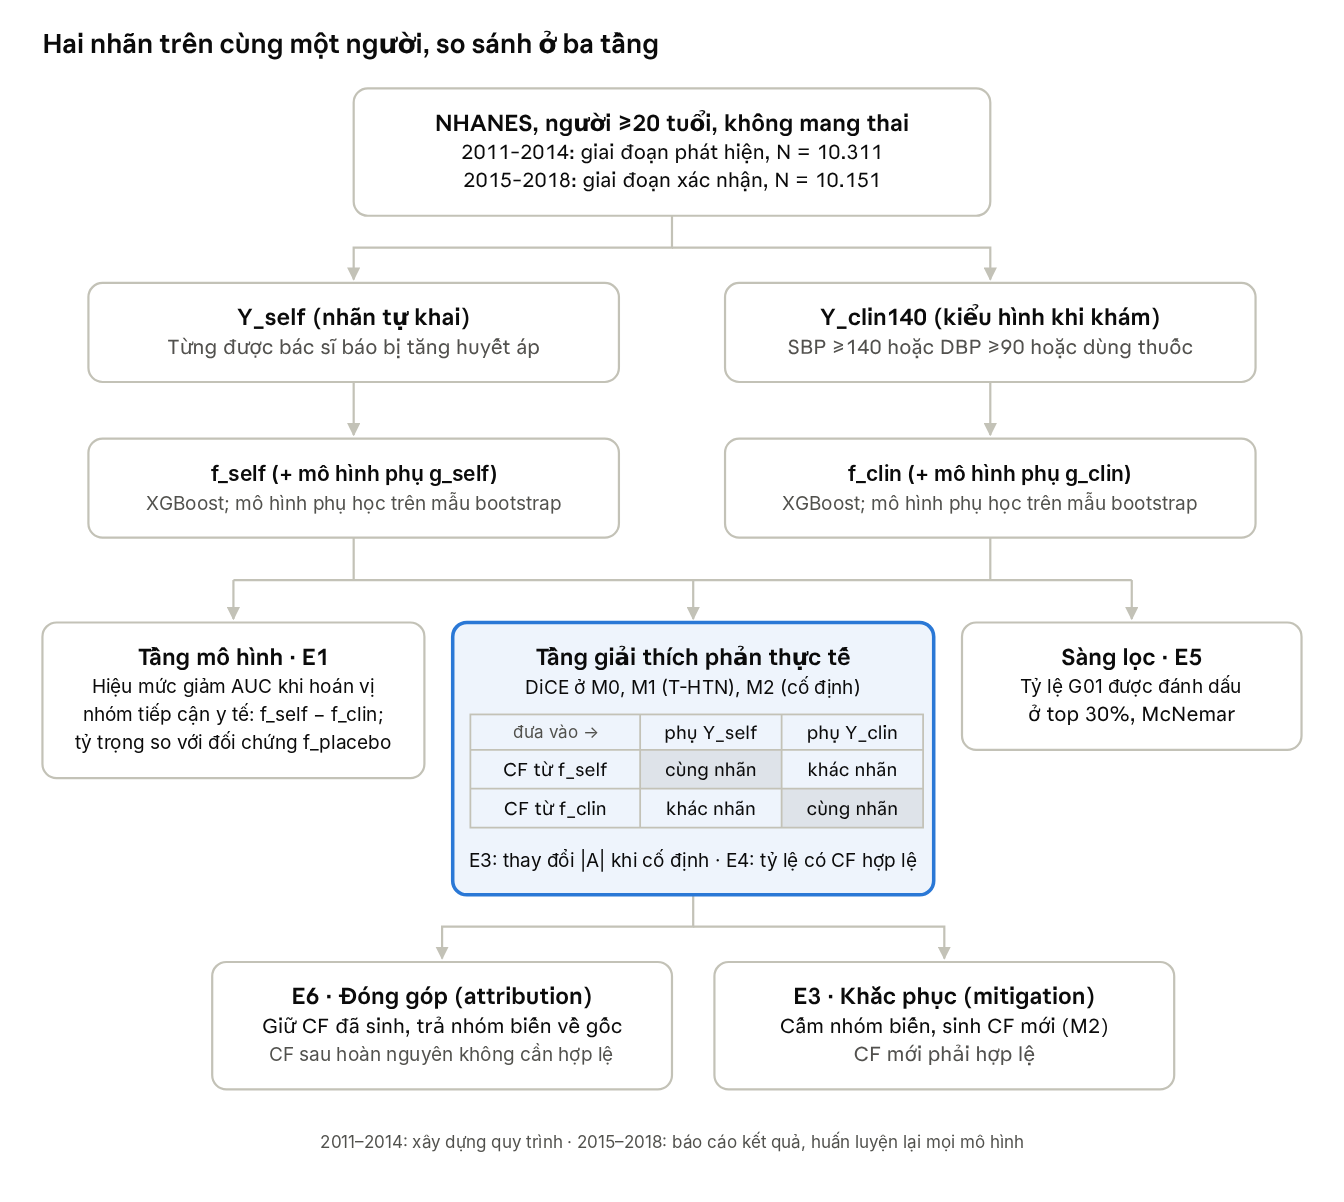
\includegraphics[width=0.66\textwidth]{fig1.png}\figcap{1}{Thiết kế quy trình kiểm định nhãn kép (PLCA). Hai mô hình chỉ khác nhau ở nhãn. Ở tầng CF, mỗi CF được đưa vào cả hai mô hình phụ để tính điểm, tạo thành ma trận 2 × 2 cùng nhãn – khác nhãn (ô tô đậm là cùng nhãn). E6 phân tích đóng góp trên các CF đã sinh; E3 đánh giá việc sinh CF mới khi cấm thay đổi nhóm biến.}\end{figure*}

Hình 1 tóm tắt thiết kế nghiên cứu. Ở mỗi tầng, hai mô hình dùng cùng
tập biến, cùng dữ liệu huấn luyện và cùng cấu hình, chỉ khác nhau ở định
nghĩa nhãn. Phép so sánh này không cho phép kết luận về quan hệ nhân quả
lâm sàng.

\begin{table*}[!t]
\tabcap{1}{Đặc điểm mẫu theo cặp nhãn, NHANES 2015–2018 (ngưỡng 140/90 mmHg).}
\begin{tabularx}{\textwidth}{>{\raggedright\arraybackslash}p{0.27\textwidth}>{\raggedleft\arraybackslash}X>{\raggedleft\arraybackslash}X>{\raggedleft\arraybackslash}X>{\raggedleft\arraybackslash}X>{\raggedleft\arraybackslash}X}
\toprule
\textbf{Đặc điểm} & \textbf{Toàn mẫu} & \textbf{G00 (cả hai −)} & \textbf{G01 (chỉ Y\_clin +)} & \textbf{G10 (chỉ Y\_self +)} & \textbf{G11 (cả hai +)} \\ \midrule
n (không trọng số) & 10.151 & 5.533 & 785 & 562 & 3.271 \\
\multicolumn{6}{l}{\textbf{Nhân khẩu học}} \\
Tuổi, năm, TB (SD) & 48,4 (17,2) & 42,1 (15,6) & 56,4 (15,3) & 44,5 (15,5) & 61,2 (13,0) \\
Tuổi 20–39, \% & 35,2 & 49,0 & 16,6 & 46,0 & 6,9 \\
Tuổi 40–59, \% & 35,8 & 35,4 & 40,5 & 34,3 & 35,8 \\
Tuổi ≥60, \% & 29,0 & 15,6 & 42,9 & 19,7 & 57,3 \\
Nữ, \% & 51,1 & 52,3 & 45,3 & 41,7 & 51,9 \\
Người Mỹ gốc Mexico, \% & 8,7 & 10,2 & 9,1 & 8,8 & 5,3 \\
Hispanic khác, \% & 6,5 & 7,2 & 6,0 & 6,8 & 5,1 \\
Da trắng không Hispanic, \% & 63,7 & 62,7 & 63,7 & 63,8 & 65,8 \\
Da đen không Hispanic, \% & 11,3 & 9,7 & 12,1 & 10,9 & 14,7 \\
Châu Á không Hispanic, \% & 5,7 & 6,3 & 5,7 & 3,8 & 4,7 \\
Khác / đa chủng tộc, \% & 4,2 & 4,0 & 3,4 & 6,0 & 4,5 \\
\multicolumn{6}{l}{\textbf{Kinh tế xã hội}} \\
Dưới THPT, \% & 12,5 & 11,5 & 13,6 & 12,2 & 14,6 \\
THPT / GED, \% & 24,2 & 22,6 & 28,0 & 24,3 & 26,8 \\
Cao đẳng / đại học chưa xong, \% & 31,7 & 30,6 & 28,1 & 35,1 & 34,3 \\
Tốt nghiệp đại học trở lên, \% & 31,6 & 35,4 & 30,3 & 28,4 & 24,3 \\
Tỷ số thu nhập/ngưỡng nghèo < 1,3, \% & 20,3 & 19,8 & 20,5 & 25,5 & 20,1 \\
\multicolumn{6}{l}{\textbf{Tiếp cận y tế}} \\
Có bảo hiểm, \% & 86,5 & 84,0 [81,2; 86,8] & 88,8 [85,2; 92,5] & 82,4 [77,2; 87,6] & 92,5 [90,4; 94,5] \\
Có nơi khám thường xuyên, \% & 82,6 & 78,0 [75,8; 80,1] & 81,8 [77,9; 85,7] & 78,7 [72,5; 84,8] & 93,9 [92,6; 95,2] \\
Có đi khám trong năm, \% & 83,9 & 79,1 [77,5; 80,7] & 78,8 [74,5; 83,0] & 82,2 [78,4; 86,0] & 96,2 [95,3; 97,0] \\
\multicolumn{6}{l}{\textbf{Sinh lý và điều trị}} \\
BMI, kg/m², TB (SD) & 29,6 (7,1) & 28,3 (6,7) & 30,3 (7,3) & 30,9 (7,4) & 32,0 (7,2) \\
SBP, mmHg, TB (SD) & 123,7 (17,7) & 115,8 (10,8) & 148,2 (13,1) & 122,0 (9,7) & 135,3 (20,0) \\
DBP, mmHg, TB (SD) & 71,7 (11,4) & 69,7 (9,1) & 82,3 (13,1) & 72,5 (10,0) & 73,2 (13,7) \\
Đang dùng thuốc hạ áp, \% & 24,1 & 0 & 0 & 0 & 89,2 \\
\bottomrule
\end{tabularx}
\tabnote{G00: cả hai nhãn âm tính; G01: kiểu hình dương tính, không cho biết đã được chẩn đoán; G10: đã được chẩn đoán, kiểu hình âm tính; G11: cả hai nhãn dương tính. Tỷ lệ và trung bình có trọng số khảo sát (WTMEC2YR chia cho số chu kỳ); n không có trọng số. Khoảng tin cậy 95\% theo thiết kế mẫu (tuyến tính hóa Taylor, 30 tầng, 60 đơn vị mẫu bậc một, ước lượng nhóm con trên toàn bộ mẫu MEC) chỉ được báo cáo cho ba biến tiếp cận y tế; các dòng còn lại là ước lượng điểm. Biến nơi khám và đi khám thiếu dữ liệu ở một người thuộc G00. Tỷ lệ dùng thuốc bằng 0 ở G00, G01 và G10 là do định nghĩa: câu hỏi về thuốc chỉ được hỏi người đã được chẩn đoán, và người đang dùng thuốc thì có Y\_clin = 1. Nguồn: results/table1/T1c\_demographics\_confirmation.csv và results/confirmation/design\_se.}
\end{table*}

\subsection{3.2. Nhãn và các nhóm không thống nhất nhãn}

Y\_self = 1 nếu người tham gia cho biết đã từng được báo là bị tăng
huyết áp. Y\_clin = 1 nếu SBP ≥140 mmHg, DBP ≥90 mmHg, hoặc đang dùng
thuốc hạ áp. Ngưỡng 140/90 mmHg là ngưỡng vận hành của nghiên cứu;
ngưỡng 130/80 mmHg theo hướng dẫn 2017 {[}4{]} được dùng trong phân tích
độ nhạy. Tình trạng dùng thuốc lấy từ hai câu hỏi BPQ040A và BPQ050A; vì
hai câu này chỉ được hỏi người đã được chẩn đoán, người chưa từng được
chẩn đoán được coi là không dùng thuốc (bỏ qua theo cấu trúc bảng hỏi),
còn người không xác định được tình trạng dùng thuốc bị loại khỏi mẫu.
Y\_clin là kiểu hình dựa trên khám, không phải ``sự thật'' (ground
truth); thành phần dùng thuốc vẫn phụ thuộc vào việc đã từng được chẩn
đoán. Theo cặp giá trị (Y\_self, Y\_clin), mỗi người thuộc một trong bốn
nhóm; G01 là nhóm có kiểu hình dương tính nhưng không cho biết đã từng
được chẩn đoán, G10 là trường hợp ngược lại.

\subsection{3.3. Biến đầu vào}

Biến đầu vào gồm sáu nhóm: nhân khẩu học và kinh tế -- xã hội; tiếp cận
y tế (bảo hiểm, có nơi khám thường xuyên, số lần đi khám); chẩn đoán
bệnh khác (tiểu đường, rối loạn mỡ máu); lối sống; chỉ số sinh lý (BMI,
vòng eo, cholesterol, HbA1c); và sức khỏe tự đánh giá (SRH). Không dùng
số đo huyết áp hay bất kỳ câu hỏi nào về huyết áp. Biến ``đã từng kiểm
tra cholesterol'' (chol\_checked, BPQ060) bị loại khỏi cấu hình chính để
nhất quán với giai đoạn phát hiện: tỷ lệ thiếu của biến này khác rõ theo
Y\_self (57,8\% ở người có Y\_self = 1 so với 26,0\% ở người có Y\_self
= 0, dữ liệu 2015--2018) do cấu trúc bỏ qua câu hỏi; phiên bản dựng lại
theo cấu trúc bảng hỏi được dùng trong phân tích độ nhạy. Ở tầng mô
hình, XGBoost xử lý trực tiếp giá trị thiếu; ở tầng CF, giá trị thiếu
được thay bằng trung vị của tập huấn luyện vì DiCE không chấp nhận giá
trị thiếu. Ba nhóm tiếp cận y tế, chẩn đoán bệnh khác và SRH được gọi
chung là \textbf{nhóm biến liên quan đến chẩn đoán}.

\subsection{3.4. Tầng mô hình (E1)}

Ba mô hình XGBoost {[}30{]} có cùng cấu hình (300 cây, độ sâu 4, tốc độ
học 0,05, tỷ lệ lấy mẫu hàng và cột 0,8), cùng tập biến và cùng dữ liệu
huấn luyện (chia 70/30, phân tầng theo Y\_clin). f\_self học Y\_self,
f\_clin học Y\_clin. Mô hình đối chứng f\_placebo học Y\_clin sau khi
nhãn bị đảo ngẫu nhiên theo hai tỷ lệ đảo lớp ước lượng từ tập huấn
luyện; nhãn nhiễu được tạo lại ở mỗi lần bootstrap. Xác suất đảo nhãn
chỉ phụ thuộc vào lớp của Y\_clin, không phụ thuộc vào các biến đầu vào.
Độ quan trọng của một nhóm biến là mức giảm AUC khi hoán vị đồng thời
mọi biến trong nhóm (trung bình ba lần hoán vị) {[}31,32{]}. Trong mỗi
lần bootstrap, các mô hình dùng chung mẫu kiểm tra và cùng thứ tự hoán
vị. Tỷ trọng của một nhóm bằng độ quan trọng của nhóm đó (giá trị âm
được đặt về 0) chia cho tổng độ quan trọng dương. Bootstrap hai tầng
{[}33{]} (B = 100) lấy mẫu lại cả tập huấn luyện lẫn tập kiểm tra, nên
khoảng ước lượng phản ánh cả biến thiên do huấn luyện lại và do lấy mẫu
kiểm tra.

\subsection{3.5. Tầng giải thích phản thực tế}

Từ tập kiểm tra, chọn tối đa 200 người không dùng thuốc và được cả hai
mô hình dự đoán dương tính (xác suất ≥0,5); nếu ít hơn 200 người thì lấy
tất cả. Ưu tiên những người có bách phân vị điểm dự đoán (trung bình của
hai mô hình) cao nhất; nhờ vậy hai mô hình dùng chung một tập người.
DiCE {[}2{]} (phiên bản 0.12, phương pháp random) được yêu cầu sinh 5 CF
cho mỗi người, theo ba chế độ; không phải người nào cũng nhận đủ 5 CF
hợp lệ:

\begin{itemize}
\tightlist
\item
  \textbf{M0:} chỉ cố định tuổi, giới tính và chủng tộc.
\item
  \textbf{M1:} taxonomy theo chiều dựa trên hướng dẫn tăng huyết áp
  (T-HTN). Tám biến được phép thay đổi theo các quy tắc kết hợp khuyến
  nghị trong hướng dẫn, cách chuyển khuyến nghị thành quy tắc trên biến
  NHANES, ràng buộc theo ngữ nghĩa dữ liệu và giả định thiết kế của
  nghiên cứu: bảo hiểm và nơi khám thường xuyên chỉ tăng; hút thuốc chỉ
  giảm; rượu chỉ giảm, tối thiểu 1 ly; vận động vừa và mạnh chỉ tăng;
  BMI chỉ giảm khi trên 25 (23 với người châu Á không gốc Tây Ban Nha)
  và không xuống dưới ngưỡng {[}34{]}; vòng eo chỉ giảm khi trên 102 cm
  (nam) hoặc 88 cm (nữ) và không xuống dưới ngưỡng {[}35,36{]}. Mọi biến
  khác cố định, kể cả sức khỏe tự đánh giá, cholesterol và HbA1c; biến
  nào bị thiếu dữ liệu rồi được điền thay cũng cố định cho người đó. Căn
  cứ của từng quy tắc ở Bảng A4.
\item
  \textbf{M2:} như M0, cố định thêm ba nhóm biến liên quan đến chẩn đoán
  (không áp dụng taxonomy).
\end{itemize}

Một CF được coi là hợp lệ khi thỏa mọi ràng buộc và làm mô hình sinh ra
nó đổi kết luận. Để đo mức tác động chéo, với mỗi nhãn có thêm một mô
hình phụ được huấn luyện trên cùng một mẫu bootstrap lấy từ tập huấn
luyện, ký hiệu g\_self và g\_clin để phân biệt với hai mô hình sinh CF
f\_self và f\_clin; mỗi CF được đưa vào cả hai mô hình phụ để tính điểm.

\textbf{Ma trận chuyển giao.} Với CF x′ của bệnh nhân i, mức giảm điểm
trên mô hình phụ g\_m là F\_m(g\_m(x\_i)) − F\_m(g\_m(x′)), trong đó
F\_m là hàm phân phối thực nghiệm của điểm g\_m trên tập kiểm tra; nhờ
vậy điểm của hai mô hình phụ được quy về cùng thang thứ hạng 0--1. Mọi
đại lượng ở tầng CF (R, ECD, A, I, E6) đều tính trên thang này; 0,01
tương ứng với 1 điểm bách phân vị. Gọi R\_sm là mức giảm trung bình khi
CF sinh từ mô hình s được đưa vào mô hình phụ m (chỉ số thứ nhất là mô
hình sinh CF, chỉ số thứ hai là mô hình phụ; s = self, c = clin). Đơn vị
phân tích là bệnh nhân: trước hết lấy trung bình trên các CF hợp lệ của
mỗi người, sau đó lấy trung bình trên mọi người trong tập phân tích. Bốn
giá trị này tạo thành ma trận 2×2 (Hình 1):

\[
\begin{array}{l|cc}
 & g_{\mathrm{self}} \text{ (học } Y_{\mathrm{self}}) & g_{\mathrm{clin}} \text{ (học } Y_{\mathrm{clin}}) \\ \hline
\text{CF từ } f_{\mathrm{self}} & R_{ss} & R_{sc} \\
\text{CF từ } f_{\mathrm{clin}} & R_{cs} & R_{cc}
\end{array}
\]

Các đại lượng chính dùng để đánh giá chuyển giao được xây dựng từ ma
trận này (tính hợp lệ và tỷ lệ tìm được CF được báo cáo riêng):

\begin{gather*}
\mathrm{ECD}_{\mathrm{self}} = R_{ss} - R_{sc}, \quad \mathrm{ECD}_{\mathrm{clin}} = R_{cc} - R_{cs} \\[3pt]
A = \mathrm{ECD}_{\mathrm{self}} - \mathrm{ECD}_{\mathrm{clin}} = (R_{ss} + R_{cs}) - (R_{sc} + R_{cc}) \\[3pt]
I = \mathrm{ECD}_{\mathrm{self}} + \mathrm{ECD}_{\mathrm{clin}} = (R_{ss} + R_{cc}) - (R_{sc} + R_{cs})
\end{gather*}

ECD (expected cross-label discrepancy, chênh lệch kỳ vọng giữa hai nhãn)
của một mô hình sinh CF là hiệu giữa hai ô trên cùng một hàng. ECD dương
nghĩa là CF làm giảm bách phân vị điểm của mô hình phụ cùng nhãn nhiều
hơn so với mô hình phụ khác nhãn. Độ bất đối xứng chuyển giao A bằng
tổng cột trái trừ tổng cột phải (A/2 là chênh lệch trung bình giữa hai
cột), tức cho biết mô hình phụ học Y\_self phản ứng mạnh hơn mô hình phụ
học Y\_clin bao nhiêu khi tính đều CF từ cả hai mô hình. Như vậy, A so
sánh hai mô hình phụ với nhau, chứ không đo riêng việc CF có ``khớp''
với mô hình phụ cùng nhãn hay không. Đại lượng đo điều đó là lợi thế
cùng nhãn I, bằng tổng đường chéo trừ tổng ngoài đường chéo (I/2 là
chênh lệch trung bình giữa ô cùng nhãn và ô khác nhãn). I dương không
đòi hỏi ECD của cả hai mô hình đều dương. I là phân tích mô tả, được bổ
sung sau khi có kết quả (Bảng A2). Việc quy về bách phân vị đưa điểm về
cùng thang thứ hạng, nhưng không bảo đảm hai mô hình phụ nhạy như nhau.
A và E6 đo chênh lệch phản ứng theo thứ hạng, không đo tác động lên nguy
cơ bệnh thật; ngoài ra, chỉ dùng một mô hình phụ cho mỗi nhãn thì chưa
loại trừ được khả năng các mô hình tương đương khác cho kết quả khác.
Công thức đầy đủ tính theo từng CF được trình bày ở Phụ lục A.

Tập phân tích: S\_M0 gồm những người có ít nhất một CF hợp lệ từ mỗi mô
hình ở chế độ M0; S* = S\_M0 ∩ S\_M2 gồm những người có CF hợp lệ từ cả
hai mô hình ở cả M0 và M2. E3 được tính trên S*, E6 trên S\_M0, và phần
ECD của E4 trên những người có CF hợp lệ từ f\_self ở cả M0 và M1.

\subsection{3.6. Tiêu chí đánh giá}

\begin{table*}[!t]
\tabcap{2}{Các tiêu chí đánh giá, câu hỏi tương ứng và vai trò.}
\begin{tabularx}{\textwidth}{>{\raggedright\arraybackslash}X>{\raggedright\arraybackslash}X>{\raggedright\arraybackslash}X>{\raggedright\arraybackslash}X}
\toprule
\textbf{Tiêu chí} & \textbf{Câu hỏi} & \textbf{Đại lượng} & \textbf{Vai trò} \\ \midrule
E1 & Phụ thuộc & Mức giảm AUC của nhóm tiếp cận y tế, f\_self − f\_clin; tỷ trọng so với f\_placebo & Chính \\
E6 & Đóng góp & Hoàn nguyên nhóm biến liên quan đến chẩn đoán trong CF ở M0; đo mức thay đổi chênh lệch phản ứng giữa hai mô hình phụ & Phụ \\
E3 & Khắc phục bằng cố định biến & A(M0) > 0, A(M0) − A(M2) > 0 và A(M0) + A(M2) > 0, tức |A| giảm khi cố định biến & Chính \\
E4 & Taxonomy dựa trên hướng dẫn có còn để lại CF hợp lệ không & Tỷ lệ có CF hợp lệ ở M1 so với M0; ECD của f\_self ở M0 trừ ở M1 khi có ít nhất 40 người chung & Mô tả \\
E5 & Hệ quả trong sàng lọc & Tỷ lệ người G01 nằm trong 30\% điểm cao nhất, kiểm định McNemar [37] & Phụ \\
\bottomrule
\end{tabularx}
\end{table*}

E6 dùng lại các CF đã sinh ở M0. Với mỗi CF x′, tạo bản hoàn nguyên
x′\_abl bằng cách trả ba nhóm tiếp cận y tế, chẩn đoán bệnh khác và SRH
về giá trị ban đầu của bệnh nhân, giữ nguyên mọi biến khác. Đóng góp của
nhóm biến trên mô hình phụ g\_m là mức điểm bách phân vị được phục hồi
khi hoàn nguyên, C\_m. E6 là trung bình của C\_self − C\_clin, lấy lần
lượt trên các CF của mỗi người, trên hai mô hình sinh CF và trên các
bệnh nhân (công thức đầy đủ ở Phụ lục A):

\begin{gather*}
C_m = F_m\big(g_m(x'_{\mathrm{abl}})\big) - F_m\big(g_m(x')\big) \\[3pt]
\mathrm{E6} = \overline{C_{\mathrm{self}} - C_{\mathrm{clin}}} = \tfrac{1}{2}\left[ A(\mathrm{M0}) - A_{\mathrm{abl}} \right]
\end{gather*}

Đẳng thức thứ hai đúng vì C\_m bằng mức giảm điểm trước trừ sau khi hoàn
nguyên, trên cùng bệnh nhân và cùng CF; A\_abl là A tính lại trên các CF
đã hoàn nguyên. Nói cách khác, E6 bằng một nửa mức giảm của A khi hoàn
nguyên nhóm biến liên quan đến chẩn đoán. CF từ hai mô hình có trọng số
bằng nhau; đơn vị phân tích là bệnh nhân. CF không thay đổi biến nào
trong nhóm thì có đóng góp bằng 0; đóng góp âm được giữ nguyên. CF sau
khi hoàn nguyên không cần còn làm mô hình sinh ra nó đổi kết luận. E6
cần ít nhất 80 người đủ điều kiện sinh CF và ít nhất 40 người có CF hợp
lệ từ cả hai mô hình ở M0; khác với E3, E6 không đòi hỏi CF hợp lệ ở M2,
bootstrap theo bệnh nhân với B = 5.000. E6 đạt khi phân vị 2,5\% dương ở
seed 42 và ước lượng điểm dương ở các seed 43, 44 đủ mẫu. E6 là tiêu chí
phụ; bài không kiểm soát sai số loại I chung (FWER) cho cả tiêu chí
chính lẫn tiêu chí phụ.

E6 là một đại lượng đo đóng góp của nhóm biến, có điều kiện theo các CF
đã sinh (counterfactual-conditioned group contribution contrast); giá
trị của nó phụ thuộc vào điểm xuất phát và các thay đổi khác trong CF.
E6 không phải giá trị Shapley, không phải quy kết nhân quả, cũng không
phải một cách phân rã dự đoán duy nhất; đóng góp của các nhóm không nhất
thiết cộng dồn được.

E6 đo đóng góp có dấu vào A; E6 dương không bảo đảm độ lớn
\textbar A\textbar{} giảm. E6 được báo cáo trên S\_M0; kết quả trên S*
chỉ dùng để đối chiếu mô tả với E3, kèm A\_abl và mức thay đổi của
\textbar A\textbar. Cần lưu ý rằng E6 sửa các CF đã có, còn E3 sinh CF
mới trong một không gian bị giới hạn; CF sau khi hoàn nguyên không cần
hợp lệ, còn CF ở M2 bắt buộc phải hợp lệ. Vì vậy, hai phép này không
phải hai cách khắc phục tương đương. Hoàn nguyên là công cụ để phân tích
đóng góp, không phải một cách sinh CF.

\subsection{3.7. Phân tích thống kê}

\begin{itemize}
\tightlist
\item
  \textbf{E1:} tiêu chí về khả năng lặp lại kết quả thực nghiệm. E1 đạt
  khi phân vị 2,5\% của chênh lệch tuyệt đối (f\_self − f\_clin) lớn hơn
  0, trung bình chênh lệch tỷ trọng so với f\_placebo lớn hơn 0, và tỷ
  trọng tính được ở ít nhất 80\% số lần bootstrap.
\item
  \textbf{E3:} bootstrap theo bệnh nhân (B = 5.000), cận dưới một phía
  là phân vị 2,5\% (α = 0,025 một phía); kiểm định giao--hợp
  (intersection--union), tức cả ba điều kiện phải cùng đạt. Khoảng
  bootstrap là có điều kiện trên tập bệnh nhân có CF hợp lệ, nên không
  bảo đảm kiểm soát chính xác sai số cho toàn bộ quy trình. Cần ít nhất
  80 người đủ điều kiện sinh CF và ít nhất 40 người trong S*.
\item
  \textbf{E4:} báo cáo mô tả, không kiểm định. ECD\_self(M0) −
  ECD\_self(M1) chỉ được diễn giải khi có ít nhất 40 người có CF hợp lệ
  từ f\_self ở cả M0 và M1; dưới ngưỡng này chỉ báo cáo tỷ lệ có CF hợp
  lệ và mức thay đổi của các biến được dùng.
\item
  \textbf{Seed:} E3, E4 và E6 được chạy với ba giá trị khởi tạo ngẫu
  nhiên (seed); các phân tích độ nhạy chỉ chạy với seed 42. Với E3 và
  E6, seed 42 là seed quyết định; ở seed 43 và 44, ước lượng điểm phải
  cùng chiều (với E3 là cả ba thành phần). Điều kiện này là nhất quán về
  hướng, không đòi hỏi ý nghĩa thống kê ở seed phụ. Nếu một seed phụ
  không đủ mẫu, tiêu chí được ghi là ``không đánh giá được độ ổn định''
  chứ không bỏ qua seed đó.
\item
  \textbf{E5 và E6:} tiêu chí phụ, ngoài nhóm kiểm định chính. Với E5,
  mỗi mô hình đánh dấu đúng round(30\% × n\_test) người có điểm cao
  nhất; nếu bằng điểm thì ưu tiên theo mã SEQN tăng dần; dùng kiểm định
  McNemar chính xác {[}37{]}, α = 0,05. Giá trị p này có điều kiện theo
  các mô hình đã huấn luyện và tập kiểm tra, không phải suy luận cho dân
  số Mỹ.
\item
  \textbf{Phạm vi suy luận:} ở tầng CF, kết luận có điều kiện theo tập
  người đã chọn, các CF hợp lệ và các mô hình đã huấn luyện.
\item
  \textbf{Bảng mô tả:} dùng trọng số khảo sát và sai số chuẩn theo thiết
  kế mẫu (phương pháp tuyến tính hóa Taylor) {[}29{]}; các mô hình không
  dùng trọng số.
\end{itemize}

\subsection{3.8. Phân tích độ nhạy}

Các phân tích sau không dùng để kết luận về tiêu chí đánh giá: ngưỡng
130/80 mmHg {[}4{]}; nhãn tự khai yêu cầu được báo có bệnh từ hai lần
trở lên; tách riêng từng chu kỳ khảo sát; so f\_self với mô hình học
huyết áp đo ở nhóm không dùng thuốc; dựng lại biến chol\_checked theo
cấu trúc bảng hỏi; hồi quy logistic; DiCE với phương pháp genetic; tập
bệnh nhân có kiểu hình dương tính; M2-phys (chỉ cố định nhóm sinh lý, để
kiểm tra tính đặc hiệu của M2); và M3 (như M1, thêm giới hạn BMI và vòng
eo giảm tối đa 5\%; mức 5\% là mục tiêu giảm cân tối thiểu trong hướng
dẫn {[}34{]}, dùng làm kịch bản).

\subsection{3.9. Môi trường tính toán và tái lập}

Toàn bộ kết quả trong bài lấy từ một lần chạy toàn bộ quy trình
(scripts/run\_all.sh) trên một máy tính xách tay chạy Linux (Intel Core
i5-1335U, 12 luồng, 16 GB RAM) với Python 3.12.3, numpy 2.5.5, pandas
3.1.1, scikit-learn 1.9.1, xgboost 3.4.1 và dice-ml 0.12. Seed 42 là
seed chính; seed 43 và 44 dùng để đánh giá độ ổn định ở tầng CF. Mỗi lần
chạy ghi lại phiên bản thư viện, commit Git và cấu hình. Việc bổ sung E6
sau khi E3 không đạt ở một lần chạy thử được khai báo ở mục 5.6. Nghiên
cứu không được đăng ký. Bài được báo cáo theo hướng dẫn TRIPOD+AI
{[}38{]}.

\section{4. Kết quả}

Trên dữ liệu 2015--2018 (Bảng 3), E1 đạt (bootstrap hai tầng B = 100,
seed 42); E3 đạt và nhất quán về hướng ở cả ba seed; E6 đạt, với cận
dưới dương ở cả ba seed; E4 cho thấy dưới T-HTN chỉ khoảng một phần mười
người còn CF hợp lệ, nên không ước lượng được hiệu quả khắc phục; E5 đạt
ở phân tích gộp nhưng không đạt khi tách từng chu kỳ. Bảng A5 tóm tắt
các tiêu chí trên cả hai giai đoạn dữ liệu. Kết quả được trình bày theo
ba phát hiện (mục 4.2--4.5); cách sắp xếp này không làm thay đổi vai trò
chính hay phụ của các tiêu chí.

\begin{table*}[!t]
\tabcap{3}{Tổng hợp kết quả các tiêu chí đánh giá, NHANES 2015–2018.}
\begin{tabularx}{\textwidth}{>{\raggedright\arraybackslash}p{0.11\textwidth}>{\raggedright\arraybackslash}p{0.19\textwidth}>{\raggedright\arraybackslash}X>{\raggedright\arraybackslash}X>{\raggedright\arraybackslash}X>{\raggedright\arraybackslash}p{0.10\textwidth}}
\toprule
\textbf{Tiêu chí (vai trò)} & \textbf{Đại lượng} & \textbf{Seed 42} & \textbf{Seed 43} & \textbf{Seed 44} & \textbf{Kết luận} \\ \midrule
E1 (chính) & Chênh lệch mức giảm AUC của nhóm tiếp cận y tế, f\_self − f\_clin; tỷ trọng so với f\_placebo & 0,014 [0,008; 0,019]; +7,0 điểm \% [2,4; 11,0] & — & — & Đạt \\
E3 (chính) & A(M0); A(M0) − A(M2); A(M0) + A(M2) & 0,120 (0,097); 0,033 (0,012); 0,208 (0,160); n = 172 & 0,058 (0,028); 0,014 (−0,009); 0,103 (0,042); n = 168 & 0,181 (0,156); 0,016 (−0,004); 0,346 (0,300); n = 175 & Đạt, nhất quán về hướng \\
E3 tính trên mọi CF (độ nhạy) & A(M0) − A(M2) & 0,011 (−0,010) & 0,004 (−0,018) & −0,012 (−0,031) & Không đạt; đổi dấu ở seed 44 \\
E4 (mô tả) & Có CF hợp lệ ở M1 so với M0, f\_self & 9,0\% so với 100\%; n chung = 18 & 12,0\% so với 99,5\%; n chung = 24 & 10,5\% so với 99,5\%; n chung = 21 & Rất ít CF hợp lệ; ECD không đủ điều kiện diễn giải (n < 40) \\
E5 (phụ) & Tỷ lệ người G01 trong 30\% điểm cao nhất, f\_self so với f\_clin & 27,8\% so với 33,3\%; p = 0,029 & — & — & Đạt ở phân tích gộp; không đạt theo từng chu kỳ \\
E6 (phụ) & Đóng góp của nhóm biến liên quan đến chẩn đoán (hoàn nguyên), trên S\_M0 & 0,043 (0,037); n = 187 & 0,044 (0,037); n = 184 & 0,058 (0,049); n = 197 & Đạt; cận dưới dương ở cả ba seed \\
\bottomrule
\end{tabularx}
\tabnote{Ngoặc tròn: cận dưới một phía (phân vị 2,5\%, bootstrap theo bệnh nhân, B = 5.000), có điều kiện theo các mô hình đã huấn luyện và tập phân tích. Ngoặc vuông: khoảng thực nghiệm 95\% từ bootstrap hai tầng (B = 100), gồm cả huấn luyện lại và lấy mẫu kiểm tra. n là số người có đủ dữ liệu trong 200 người được chọn. E1 và E5 chỉ được đánh giá ở seed 42. Ở seed 43 và 44, ước lượng phải cùng chiều (với E3 là cả ba thành phần); E3 dùng tập S* riêng của từng seed; ở seed 43 và 44, cận dưới của A(M0) − A(M2) âm nhưng ước lượng điểm cùng chiều, nên E3 vẫn đạt điều kiện nhất quán về hướng.}
\end{table*}

\subsection{4.1. Đặc điểm mẫu}

Trong 10.151 người, hai nhãn không thống nhất ở 12,9\% {[}11,8; 13,9{]}
(có trọng số, sai số theo thiết kế mẫu); với ngưỡng 130/80 mmHg, tỷ lệ
này là 23,1\% {[}21,8; 24,3{]}. So với nhóm G11 (đã được chẩn đoán),
nhóm G01 (kiểu hình dương tính nhưng không cho biết đã được chẩn đoán)
ít có nơi khám thường xuyên và ít đi khám hơn hẳn, với khoảng tin cậy
không chồng lên nhau; khác biệt về bảo hiểm nhỏ hơn. So với nhóm cả hai
nhãn đều âm tính (G00), nhóm G01 lớn tuổi hơn (trung bình 56,4 so với
42,1 tuổi), có tỷ lệ nữ thấp hơn (45,3\% so với 52,3\%) và huyết áp
trung bình 148/82 mmHg; phân bố chủng tộc, học vấn và thu nhập gần với
toàn mẫu (Bảng 1).

\subsection{4.2. Phát hiện 1: mức phụ thuộc vào nhóm biến liên quan đến
chẩn đoán khác nhau theo nguồn nhãn (E1)}

f\_self và f\_clin có AUC trên tập kiểm tra gần nhau (0,806 và 0,831;
hai giá trị được tính trên hai nhãn khác nhau) nhưng dựa vào những nhóm
biến khác nhau.

\begin{figure}[!t]\centering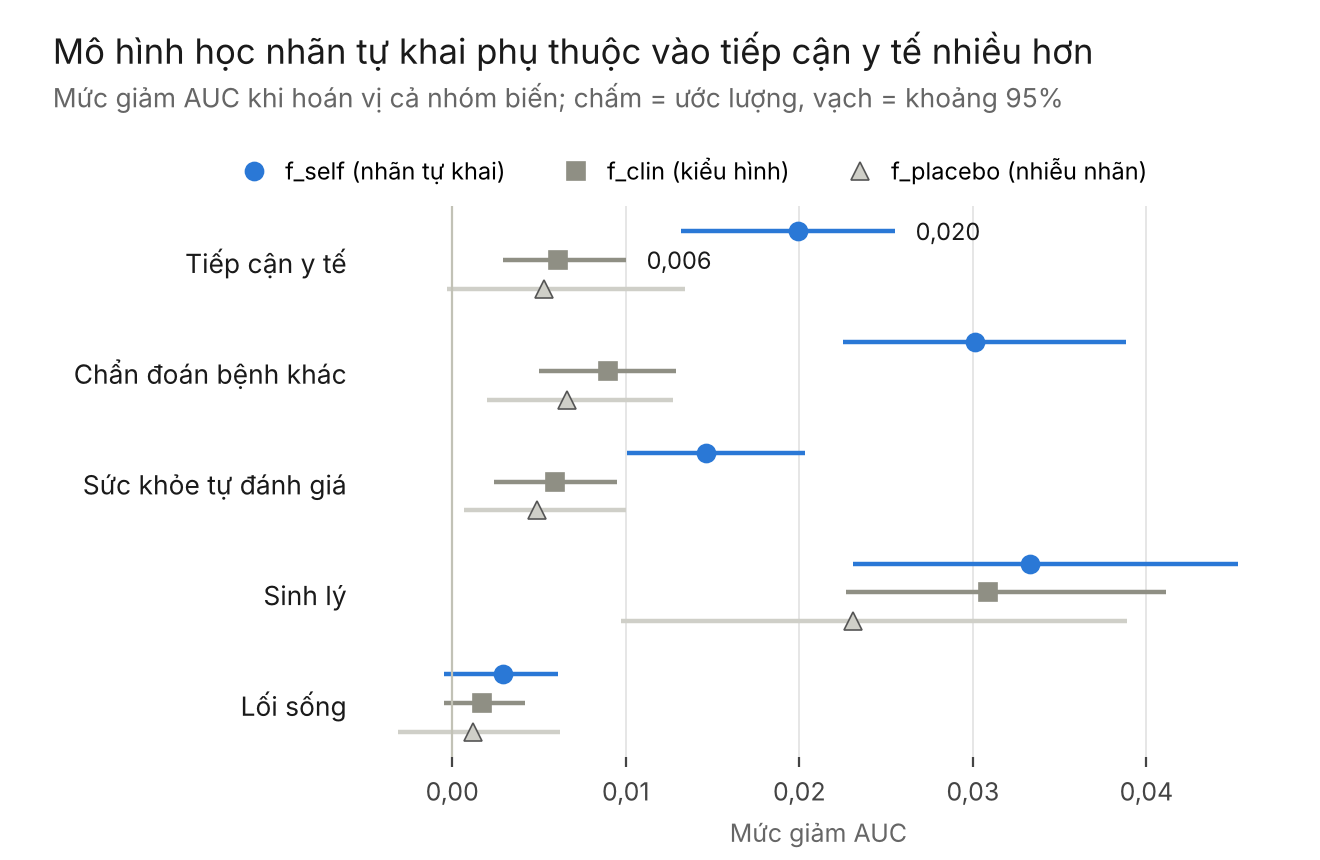
\includegraphics[width=\columnwidth]{fig2.png}\figcap{2}{Mức giảm AUC khi hoán vị từng nhóm biến ở ba mô hình (NHANES 2015–2018, seed 42, bootstrap hai tầng B = 100). Chấm là ước lượng điểm, vạch là khoảng 95\%. Không vẽ nhóm nhân khẩu học (f\_self 0,103; f\_clin 0,211).}\end{figure}

Mức giảm AUC khi hoán vị nhóm tiếp cận y tế ở f\_self cao hơn ở f\_clin
0,014 {[}0,008; 0,019{]}; tỷ trọng của nhóm này trong tổng độ quan trọng
cũng cao hơn so với f\_placebo 7,0 điểm phần trăm {[}2,4; 11,0{]} (9,8\%
so với 2,8\%). Mô hình đối chứng nhiễu nhãn không tạo ra được mức phụ
thuộc này. Nhóm chẩn đoán bệnh khác và nhóm sức khỏe tự đánh giá cho xu
hướng tương tự, còn nhóm sinh lý có độ quan trọng khá gần nhau ở hai mô
hình (0,033 và 0,031). Ngược lại, nhóm nhân khẩu học -- kinh tế xã hội
quan trọng hơn ở f\_clin (0,211 so với 0,103), nên khác biệt giữa hai mô
hình không chỉ nằm ở nhóm tiếp cận y tế; đây là mô tả, không cho phép
suy ra cơ chế. Kết quả này giống với giai đoạn phát hiện (0,015
{[}0,009; 0,022{]}). Khi loại nhóm G01 khỏi tập huấn luyện, chênh lệch
giảm còn 0,005 {[}0,000; 0,010{]}, so với 0,014 khi loại ngẫu nhiên cùng
số người (phân tích mô tả).

Phát hiện này có giới hạn rõ ràng. Khi so f\_self với mô hình học huyết
áp đo ở nhóm không dùng thuốc, chênh lệch về tiếp cận y tế không lặp
lại: −0,003 {[}−0,017; 0,011{]}, và −0,003 {[}−0,017; 0,009{]} ở giai
đoạn phát hiện. Khoảng tin cậy chứa 0 nghĩa là không xác nhận được chênh
lệch, chứ không chứng minh hai mô hình phụ thuộc như nhau. Vì vậy, mức
phụ thuộc vào biến tiếp cận y tế gắn với cách định nghĩa kiểu hình và
quần thể được xét.

\subsection{4.3. Phát hiện 2a: nhóm biến liên quan đến chẩn đoán đóng
góp vào khác biệt phản ứng giữa hai mô hình (E6)}

Khi hoàn nguyên nhóm biến liên quan đến chẩn đoán, điểm của mô hình phụ
học nhãn tự khai tăng trở lại nhiều hơn so với mô hình phụ học kiểu
hình: E6 = 0,043 (cận dưới 0,037; 187 người). Kết quả ở seed 43 và 44
cùng chiều (0,044 và 0,058). Hiệu ứng xuất hiện với CF từ cả hai mô hình
(0,057 và 0,030). Trên S\_M0, 49--65\% CF hợp lệ có thay đổi ít nhất một
biến thuộc nhóm này (tùy mô hình sinh CF và seed).

\begin{table}[!t]
\tabcap{4}{Đóng góp của từng nhóm biến khi hoàn nguyên riêng (E6, seed 42).}
\begin{tabularx}{\columnwidth}{>{\raggedright\arraybackslash}X>{\raggedright\arraybackslash}X}
\toprule
\textbf{Nhóm được hoàn nguyên (seed 42)} & \textbf{Đóng góp} \\ \midrule
Tiếp cận y tế & 0,020 \\
Chẩn đoán bệnh khác & 0,017 \\
Sức khỏe tự đánh giá & 0,007 \\
\bottomrule
\end{tabularx}
\tabnote{Đóng góp của các nhóm không cộng dồn được vì các biến tương tác với nhau. Thứ hạng ba nhóm thay đổi giữa các seed: tiếp cận y tế lớn nhất ở seed 42; SRH lớn nhất ở seed 43 (0,022); chẩn đoán bệnh khác lớn nhất ở seed 44 (0,031). Nhóm tiếp cận y tế đóng góp đáng kể ở cả ba seed nhưng không phải lúc nào cũng lớn nhất.}
\end{table}

\subsection{4.4. Phát hiện 2b: cố định nhóm biến đó khi sinh CF chỉ giảm
được một phần khác biệt ở 2015--2018 (E3)}

Trên 172 người có CF hợp lệ từ cả hai mô hình ở cả hai chế độ, A(M0) =
0,120 (cận dưới 0,097). Khi cố định nhóm biến liên quan đến chẩn đoán, A
giảm còn 0,087; hiệu số 0,033 có cận dưới 0,012, và điều kiện về độ lớn
có cận dưới 0,160. Ước lượng điểm của cả ba thành phần đều dương ở seed
43 và 44, nên E3 đạt và nhất quán về hướng; tuy nhiên biên an toàn mỏng,
vì ở hai seed này cận dưới của hiệu số A(M0) − A(M2) âm (−0,009 và
−0,004). Tuy nhiên, khi tính trên mọi CF mà DiCE trả về (kể cả CF không
làm mô hình sinh ra nó đổi kết luận), E3 không đạt ở cả ba seed (Bảng
3): hiệu số nhỏ hơn ở cả ba seed và đổi dấu ở seed 44 (−0,012). Trên dữ
liệu 2011--2014, E3 không đạt, và A(M2) đổi dấu ở seed 42 và 43 (−0,032
và −0,037). Ở seed 42, độ lớn của A giảm khoảng 20\%, nhưng cận dưới
bootstrap của A(M0) + A(M2) âm (−0,028). Ở seed 43, độ lớn của A tăng
khoảng 26\%. Ở seed 44, độ lớn của A giảm khoảng 51\% (Bảng A5). Như
vậy, tác động của việc cố định nhóm biến không ổn định giữa các giai
đoạn và các seed, và kết quả nhạy với cách chọn CF đưa vào phân tích;
hai cách tính cũng dùng tập CF và tập người khác nhau, nên không thể quy
toàn bộ khác biệt cho bước lọc CF hợp lệ.

\begin{figure}[!t]\centering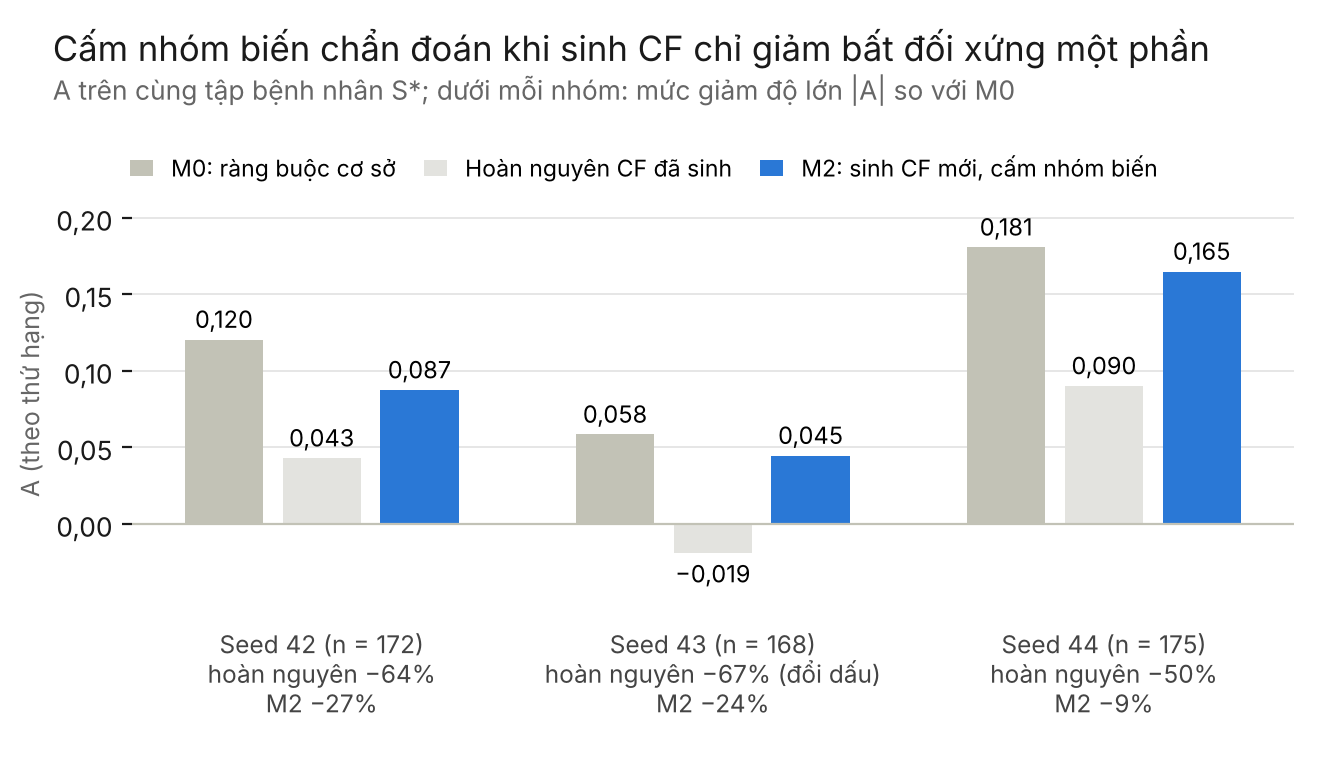
\includegraphics[width=\columnwidth]{fig3.png}\figcap{3}{Độ bất đối xứng chuyển giao A trên cùng tập bệnh nhân S* ở mỗi seed: CF với ràng buộc cơ sở (M0), CF đã sinh sau khi hoàn nguyên, và CF sinh mới khi cấm thay đổi nhóm biến (M2). Mức giảm dưới mỗi nhóm tính theo độ lớn |A|; ở seed 43, A đổi dấu sau khi hoàn nguyên.}\end{figure}

Hình 3 thể hiện điểm mấu chốt của bài. Khi sửa các CF đã có bằng cách
trả nhóm biến liên quan đến chẩn đoán về giá trị ban đầu, độ lớn của bất
đối xứng, \textbar A\textbar, giảm 50--67\% (giảm tuyệt đối
0,039--0,091); ở seed 43, A còn đổi dấu sau khi hoàn nguyên (từ 0,058
xuống −0,019). Nhưng khi cấm hẳn các biến đó và để DiCE tìm CF mới, độ
lớn bất đối xứng chỉ giảm 9--27\% (giảm tuyệt đối 0,014--0,033), phù hợp
với giả thuyết rằng thuật toán đã chuyển sang dùng các biến khác. Khoảng
cách giữa hai mức giảm chỉ mang tính mô tả; không có tiêu chí riêng để
kiểm định nó. Hai thành phần của A thay đổi theo hai hướng khác nhau
(seed 42): ECD của f\_self giảm từ 0,089 xuống 0,070, còn ECD của
f\_clin tăng từ −0,031 lên −0,018. ECD của f\_clin ở M0 âm ở seed 42 và
44, dương nhẹ ở seed 43. A dương nghĩa là, khi tính đều CF từ hai mô
hình, mô hình phụ học Y\_self phản ứng mạnh hơn. Bảng A2 trình bày từng
thành phần trên S*. Ở M0, I dương (0,058; 0,088; 0,070), tức có lợi thế
cùng nhãn khi gộp CF từ hai mô hình, dù điều này không nhất thiết đúng
với từng mô hình riêng lẻ. Khi cố định biến, A giảm nhưng I không giảm
một cách nhất quán (0,052; 0,114; 0,144: giảm nhẹ ở seed 42, tăng ở seed
43 và 44). Đây là mô tả bổ sung, không có khoảng tin cậy: giảm chênh
lệch giữa hai mô hình phụ không đồng nghĩa với giảm lợi thế cùng nhãn.
Bảng A3 mô tả phản ứng tính theo từng CF, với tập dữ liệu và cách lấy
trung bình khác Bảng A2.

\subsection{4.5. Phát hiện 3: taxonomy dựa trên hướng dẫn gần như không
còn CF hợp lệ (E4)}

Dưới T-HTN, chỉ 9,0--12,0\% người có CF hợp lệ từ f\_self và 3,0--7,5\%
từ f\_clin, so với 92--100\% ở M0 và 86--99\% ở M2 (Hình 4). Mọi người
đều còn ít nhất một biến được phép thay đổi; phần lớn trường hợp thất
bại là DiCE không tìm được CF (88--97\%). Số người có CF hợp lệ ở cả M0
và M1 chỉ là 18, 24 và 21 ở ba seed, dưới ngưỡng 40, nên phần ECD của E4
không được diễn giải. Mọi CF hợp lệ dưới T-HTN đều giảm BMI hoặc vòng
eo, và mức giảm thường lớn: BMI giảm trung bình 27--37\% so với giá trị
ban đầu, và 74--94\% CF giảm BMI hơn 10\% (tính trên các CF hợp lệ, vốn
rất ít). Không CF hợp lệ nào thay đổi biến tiếp cận y tế, dù các biến
này được phép tăng.

\begin{figure}[!t]\centering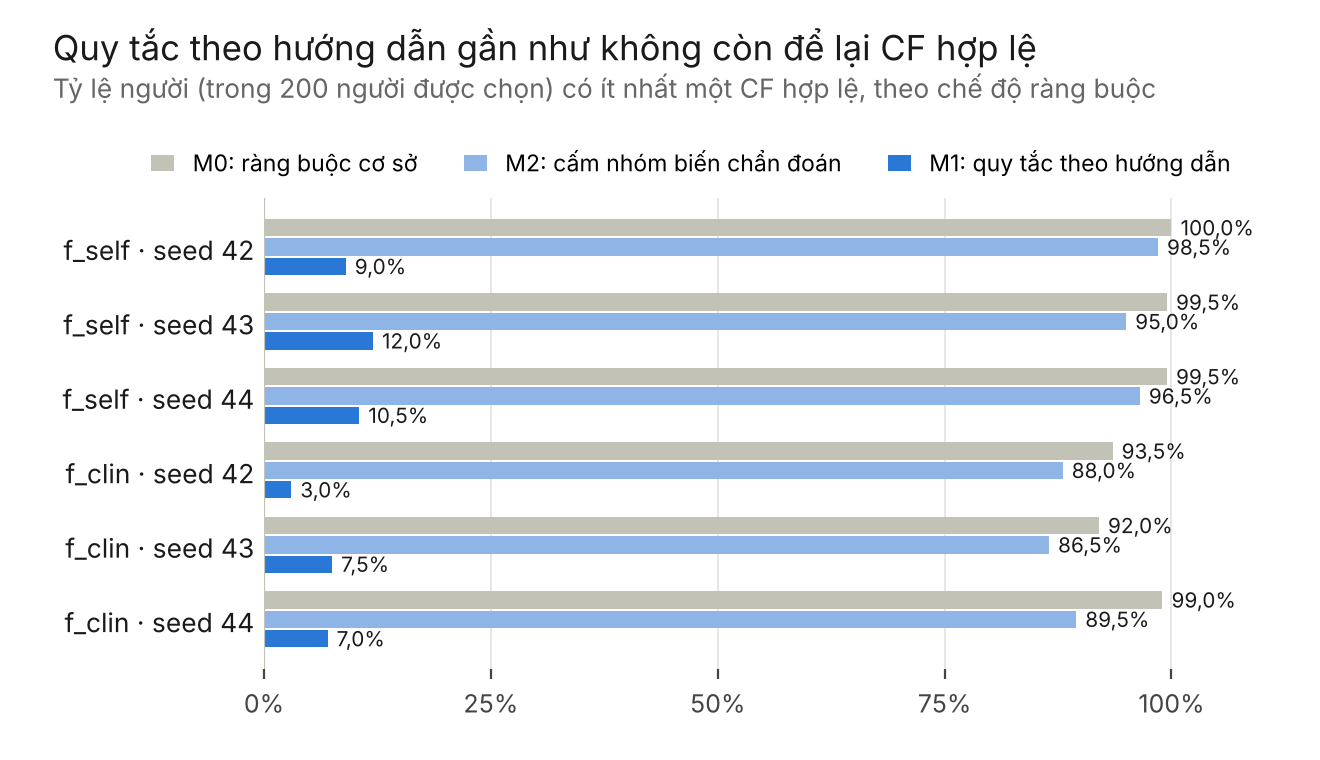
\includegraphics[width=\columnwidth]{fig4.png}\figcap{4}{Tỷ lệ người có ít nhất một CF hợp lệ ở M0 (ràng buộc cơ sở), M2 (cấm nhóm biến liên quan đến chẩn đoán) và M1 (T-HTN), theo mô hình sinh CF và seed (200 người được chọn ở mỗi seed).}\end{figure}

\subsection{4.6. Kết quả phụ: hệ quả trong sàng lọc (E5)}

Với ngân sách sàng lọc 30\%, f\_self xếp 27,8\% người G01 vào nhóm điểm
cao, so với 33,3\% của f\_clin (11 so với 25 trường hợp chỉ một mô hình
đánh dấu; p = 0,029), nên E5 đạt ở phân tích gộp. Tuy nhiên, khi tách
riêng từng chu kỳ, khác biệt không đạt ý nghĩa (p = 0,21 ở 2015--2016 và
0,115 ở 2017--2018); vì cỡ mẫu mỗi chu kỳ nhỏ hơn, điều này không cho
thấy hiệu ứng không tồn tại, nhưng kết quả cần được diễn giải thận
trọng. Ngoài ra, nhóm G01 được xác định một phần bằng chính nhãn mà
f\_clin học, nên E5 là mô tả hệ quả, không phải bằng chứng độc lập về
lợi ích lâm sàng. Ở ngưỡng xác suất 0,5, khác biệt rõ hơn (35,3\% so với
49,0\%; p \textless{} 0,001), nhưng đây không phải tiêu chí của E5.

\subsection{4.7. Phân tích độ nhạy}

\begin{table}[!t]
\tabcap{5}{Phân tích độ nhạy cho E1, E3 và E6 (NHANES 2015–2018). Các phân tích này không dùng để kết luận về tiêu chí đánh giá. Ở tầng CF, phân tích độ nhạy chỉ chạy với seed 42, nên "đạt" nghĩa là thỏa điều kiện ở seed chính, không phải đạt và nhất quán về hướng. Số người trong ngoặc cho thấy E6 giữ được nhiều người hơn E3, vì E6 không đòi hỏi việc sinh CF có ràng buộc thành công.}
\begin{tabularx}{\columnwidth}{>{\raggedright\arraybackslash}X>{\raggedright\arraybackslash}X>{\raggedright\arraybackslash}X>{\raggedright\arraybackslash}X}
\toprule
\textbf{Phân tích} & \textbf{E1} & \textbf{E3} & \textbf{E6} \\ \midrule
Ngưỡng 130/80 mmHg & 0,019, đạt & — & — \\
Nhãn tự khai (được báo ≥2 lần) & 0,017, đạt & — & — \\
Từng chu kỳ 2015–2016 / 2017–2018 & 0,011 / 0,015, đạt & — & — \\
f\_self so với f\_bp, nhóm không dùng thuốc & −0,003, \textbf{không đạt} & — & — \\
Hồi quy logistic & 0,008, đạt & đạt (88 người) & 0,085 (191 người) \\
DiCE genetic & — & đạt (177 người) & 0,105 (192 người) \\
Tập bệnh nhân có kiểu hình dương tính & — & đạt (104 người) & 0,033 (109 người) \\
Tính trên mọi CF & — & \textbf{không đạt} & — \\
\bottomrule
\end{tabularx}
\end{table}

M2-phys (chỉ cố định nhóm sinh lý) làm A tăng từ 0,137 lên 0,191 trên 89
người chung, trong khi M2 làm A giảm. Trên cùng 89 người này, hiệu số
A(M0) − A(M2) là 0,032 {[}0,003; 0,062{]}, nên kết quả ủng hộ tính đặc
hiệu tương đối của M2; tuy vậy, hai cách cố định khác nhau về số biến và
vai trò dự đoán. Với M3, chỉ 0,5\% (f\_self) và 0\% (f\_clin) bệnh nhân
có CF hợp lệ. Trong hồi quy logistic, không có cặp hệ số nào trái dấu rõ
rệt giữa hai nhãn; khác biệt chủ yếu nằm ở độ lớn (ví dụ, hệ số của số
lần đi khám là 0,21 so với 0,10).

Với DiCE genetic, A giảm từ 0,242 (M0) xuống 0,169 (M2), tức giảm 30\%,
gần với mức 27\% của DiCE random; nhưng A ở M0 lớn gần gấp đôi, cho thấy
độ lớn của bất đối xứng phụ thuộc vào thuật toán sinh CF. Khi đưa lại
biến chol\_checked đã dựng lại, E1 = 0,016 {[}0,008; 0,023{]}, vẫn đạt.

\section{5. Bàn luận}

\subsection{5.1. Ba khái niệm không nên đánh đồng}

Hai mô hình có hiệu năng gần nhau vẫn có thể dựa vào những yếu tố khác
nhau và sinh ra những CF khác nhau, chỉ vì nhãn được tạo ra theo cách
khác. Bản thân điều này không có gì bất ngờ. Đóng góp của bài nằm ở việc
tách bạch ba đại lượng mà các nghiên cứu ứng dụng AI giải thích được
(XAI) dễ đánh đồng.

\begin{enumerate}
\def\labelenumi{\arabic{enumi}.}
\tightlist
\item
  \textbf{Phụ thuộc ở tầng mô hình khác với đóng góp trong CF.} E1 đo
  mức mô hình dựa vào nhóm tiếp cận y tế trên toàn bộ dữ liệu; E6 đo
  đóng góp của những thay đổi thuộc nhóm biến liên quan đến chẩn đoán
  (gồm tiếp cận y tế, chẩn đoán bệnh khác và SRH) trong các CF cụ thể.
  Hai đại lượng liên quan với nhau nhưng không cùng nhóm biến và không
  cùng estimand. Một nhóm biến quan trọng với mô hình có thể ít xuất
  hiện trong CF, và ngược lại. Trong nghiên cứu này, hai đại lượng cùng
  chiều (mô hình học nhãn tự khai dựa vào tiếp cận y tế nhiều hơn, và
  nhóm biến liên quan đến chẩn đoán đóng góp vào khác biệt phản ứng),
  nhưng bài không kiểm định trực tiếp sự khác nhau giữa chúng; đây là
  phân biệt về mặt khái niệm, có ý nghĩa cho việc thiết kế quy trình
  kiểm định. Mức phụ thuộc ở tầng mô hình cũng có giới hạn: nó không lặp
  lại khi so với nhãn chỉ dựa trên huyết áp đo ở nhóm không dùng thuốc.
\item
  \textbf{Đóng góp khác với khắc phục.} Đây là phát hiện chính (mục
  5.2).
\item
  \textbf{Hợp lý chưa chắc còn tìm được CF.} Một taxonomy dựa trên hướng
  dẫn điều trị chặn được các đề xuất ngược chiều, nhưng gần như không
  còn CF hợp lệ (mục 5.3).
\end{enumerate}

\subsection{5.2. Đóng góp không đồng nghĩa với khắc phục được}

Ở seed 42, hoàn nguyên trên các CF đã sinh làm \textbar A\textbar{} giảm
64\% (50--67\% ở ba seed, kèm đổi dấu ở seed 43), trong khi sinh CF với
nhóm biến bị cố định chỉ làm \textbar A\textbar{} giảm 27\% (9--27\%);
các con số này thuộc giai đoạn 2015--2018. Ở 2011--2014, tác động của
việc cố định không ổn định cả về độ lớn lẫn chiều của A. Mức giảm được
tính theo độ lớn, 100 × (\textbar A(M0)\textbar{} − \textbar A\textbar)
/ \textbar A(M0)\textbar; so sánh theo mức giảm tuyệt đối cũng cho cùng
kết luận (Hình 3). Bài tính theo độ lớn vì cùng lý do E3 có điều kiện
A(M0) + A(M2) \textgreater{} 0: phân biệt giảm độ lớn với đảo chiều. Đây
là so sánh mô tả; không có tiêu chí riêng để kiểm định khoảng cách này.
Hai phép phân tích khác nhau cả về mục đích lẫn điều kiện hợp lệ. Khi bị
ràng buộc, thuật toán sinh CF có thể tìm tổ hợp thay đổi khác, nhưng
nghiên cứu chưa xác định được cơ chế thay thế cụ thể. M2-phys cho phép
đối chiếu tính đặc hiệu tương đối, nhưng không chứng minh nguyên nhân.
Xét theo cấu tạo đại số của A, phần được giảm là chênh lệch phản ứng
giữa hai mô hình phụ, còn I không giảm một cách nhất quán (Bảng A2, mô
tả). Đóng góp đo được trên các CF đã sinh không dự báo trực tiếp hiệu
quả khắc phục. Bài học có tính khái quát hơn con số cụ thể là: cần đánh
giá riêng phép phân tích đóng góp và việc sinh CF có ràng buộc, thay vì
suy ra hiệu quả của cách thứ hai từ kết quả của cách thứ nhất.

\subsection{5.3. Ràng buộc theo hướng dẫn và khả năng tìm được CF}

T-HTN kết hợp các chiều thay đổi được hỗ trợ bởi hướng dẫn y khoa, quy
tắc chuyển đổi trên biến NHANES, ràng buộc theo ngữ nghĩa dữ liệu và giả
định thiết kế, và giữ cố định các chỉ báo trạng thái như sức khỏe tự
đánh giá. Kết quả là khoảng chín phần mười người được cả hai mô hình dự
đoán dương tính không còn CF hợp lệ trong ngân sách tìm kiếm của DiCE.
Cố định biến (M2) và ràng buộc theo chiều (M1) vì vậy cho thấy hai giới
hạn khác nhau của việc khắc phục bằng ràng buộc: M2 còn tìm được CF
nhưng tác động lên khác biệt không ổn định (chỉ giảm một phần ở
2015--2018), còn M1 có căn cứ hướng dẫn rõ hơn và ràng buộc chặt hơn,
nhưng gần như không còn CF để đánh giá. Ngay cả các CF hợp lệ dưới M1
cũng thường đòi giảm BMI hơn 10\%; thỏa ràng buộc về chiều không bảo đảm
biên độ thay đổi hợp lý, và khi giới hạn thêm biên độ (M3) thì gần như
không còn CF nào. Việc không CF hợp lệ nào dùng biến tiếp cận y tế theo
chiều tăng ở giai đoạn 2015--2018 (ở 2011--2014, chỉ 1,2\% CF hợp lệ của
f\_self ở seed 42 thay đổi bảo hiểm) có thể phù hợp với nhận định rằng
mô hình dùng các biến này như dấu hiệu của việc đã được chẩn đoán, nhưng
kết quả này không xác định được cơ chế, vì còn phụ thuộc vào giá trị ban
đầu (nhiều người đã có bảo hiểm), ràng buộc của từng người và thuật toán
tìm kiếm. Tỷ lệ tìm được CF thấp không chứng minh rằng không tồn tại
thay đổi nào làm mô hình đổi kết luận; nó phụ thuộc vào thuật toán (ở
đây là DiCE random), số CF yêu cầu, ngân sách tìm kiếm, cũng như các mô
hình và tập người được chọn của nghiên cứu.

\subsection{5.4. Ý nghĩa đối với hệ hỗ trợ quyết định lâm sàng}

\begin{enumerate}
\def\labelenumi{\arabic{enumi}.}
\tightlist
\item
  Khi có dữ liệu với hai nhãn, nên kiểm định nguồn nhãn trước khi đưa CF
  vào sử dụng. AUC gần nhau không bảo đảm lời giải thích giống nhau.
\item
  Chẩn đoán bệnh khác và sức khỏe tự đánh giá nên được xem là chỉ báo
  trạng thái, không phải mục tiêu can thiệp.
\item
  Cố định nhóm biến liên quan đến chẩn đoán có tác động không ổn định
  lên khác biệt phản ứng giữa hai mô hình phụ (chỉ giảm một phần ở
  2015--2018, không đạt tiêu chí ở 2011--2014); taxonomy dựa trên hướng
  dẫn làm giảm mạnh tỷ lệ tìm được CF hợp lệ, nên chưa đánh giá được
  hiệu quả khắc phục của nó. Nên báo cáo cả mức thay đổi điểm của mô
  hình dưới từng ràng buộc, không chỉ tỷ lệ CF làm đổi kết luận.
\item
  Khi chỉ cho phép thay đổi có căn cứ hướng dẫn (M1), và nhất là khi
  giới hạn thêm biên độ (M3), rất ít người có CF hợp lệ. Không tìm được
  CF trong ngân sách tìm kiếm chưa chứng minh người bệnh không thể thay
  đổi kết quả; nó chỉ cho thấy tỷ lệ tìm được CF thấp với các giới hạn
  và ngân sách đã định.
\end{enumerate}

\textbf{Điều kiện áp dụng PLCA.} Quy trình có thể dùng lại cho bài toán
khác khi: (i) có hai định nghĩa kết cục được ghi nhận trên cùng một
người; (ii) hai nhiệm vụ dùng chung một tập đặc trưng; (iii) có thể huấn
luyện các mô hình phân loại với cùng cấu hình; và (iv) xác định được
trước nhóm biến cần kiểm định và cách sinh CF tương ứng. Chiều của tiêu
chí E3 là giả thuyết riêng cho nghiên cứu tăng huyết áp này; bản thân
PLCA không đòi hỏi A ban đầu luôn dương, và ở bài toán khác các tiêu chí
cần được xác định lại theo dữ liệu phát hiện. Nghiên cứu này chưa kiểm
chứng PLCA trên bệnh hay bộ dữ liệu khác.

\subsection{5.5. So sánh với các nghiên cứu trước}

Kết quả phù hợp với giả thuyết về biến đại diện (proxy) của Thieu
{[}9{]}, trên một bệnh và một bộ dữ liệu khác; taxonomy của bài dựa trên
hướng dẫn tăng huyết áp thay vì ADA, và bài không kiểm định trực tiếp
taxonomy tiểu đường gốc. Cerrato và cộng sự {[}10{]} nghiên cứu sự thay
đổi của tập CF khi đổi định nghĩa nhãn; PLCA bổ sung việc đánh giá cùng
một CF trên hai mô hình phụ, và phân tích riêng phép hoàn nguyên với
việc sinh CF có cố định biến. Mothilal và cộng sự {[}24{]} đã khảo sát
quan hệ giữa quy kết và việc giới hạn đặc trưng; điểm mới ở đây là bối
cảnh hai nhãn và đại lượng đo phản ứng chéo giữa hai mô hình phụ. Trong
hồi quy logistic, không có cặp hệ số nào trái dấu rõ rệt; đây chỉ là mô
tả, không phải kiểm định lý thuyết của Zanger-Tishler và cộng sự
{[}11{]}.

\subsection{5.6. Hạn chế và các yếu tố ảnh hưởng đến tính giá trị}

\begin{itemize}
\tightlist
\item
  \textbf{Dữ liệu và nhãn:} thiết kế cắt ngang; Y\_self phản ánh việc đã
  từng được chẩn đoán trong quá khứ, còn Y\_clin là huyết áp tại thời
  điểm khảo sát hoặc việc đang dùng thuốc. Khác biệt giữa hai nhãn vì
  vậy bao gồm cả cách ghi nhận lẫn khung thời gian của kết cục, không
  thể quy riêng cho tiếp cận y tế. Không có nhãn ``sự thật''.
\item
  \textbf{Khả năng khái quát:} chỉ một bệnh và một nguồn dữ liệu của Mỹ;
  các mô hình là phương tiện thực nghiệm, chưa được đánh giá về lợi ích
  lâm sàng. Áp dụng cho các bệnh khác có hai nhãn (ví dụ tiểu đường tự
  khai so với HbA1c) là hướng kiểm chứng tiếp theo.
\item
  \textbf{Nhóm không dùng thuốc:} khi so với nhãn chỉ dựa trên huyết áp
  đo, E1 không lặp lại ở cả hai giai đoạn; kết quả phụ thuộc vào quần
  thể và cách định nghĩa kiểu hình.
\item
  \textbf{Độ ổn định:} E3 nhạy với seed và cách chọn CF; ở giai đoạn
  2015--2018, E3 chỉ nhất quán về hướng chứ không có cận dưới dương ở
  seed phụ; ở seed 43 và 44, cận dưới của A(M0) − A(M2) âm dù ước lượng
  điểm dương; trên dữ liệu 2011--2014, E3 không đạt. E5 đạt ở phân tích
  gộp nhưng không đạt khi tách từng chu kỳ. Như mọi nghiên cứu học máy,
  kết quả có thể thay đổi nhẹ giữa các môi trường tính toán do sai số số
  học và tính ngẫu nhiên của thuật toán sinh CF.
\item
  \textbf{Suy luận ở tầng CF:} kết luận có điều kiện theo tập người được
  chọn, các CF hợp lệ và các mô hình đã huấn luyện. Chỉ một mô hình phụ
  cho mỗi nhãn là đối chứng có giới hạn; ba seed không phải ba lần xác
  nhận độc lập. Việc quy về bách phân vị không loại bỏ hết khác biệt về
  độ nhạy giữa hai mô hình.
\item
  \textbf{Phương pháp:} các mô hình không dùng trọng số khảo sát.
  Taxonomy và các giới hạn biên độ chưa được chuyên gia thẩm định và
  không biểu diễn được các khuyến nghị về natri, kali, chế độ ăn DASH và
  quản lý căng thẳng, vì các yếu tố này không có trong tập biến; CF
  không phải lời khuyên y khoa. Nghiên cứu không được đăng ký.
\item
  \textbf{Tiêu chí phụ và phân tích bổ sung:} E6 được thêm vào trong
  giai đoạn phát hiện, sau khi E3 không đạt ở một lần chạy thử; định
  nghĩa và vai trò của E6 được xác định trước khi tính trên dữ liệu
  2015--2018. I là phân tích mô tả bổ sung; bài không thêm kiểm định hay
  tiêu chí mới.
\end{itemize}

\textbf{Tóm tắt phạm vi kết luận.} Bảng A1 (Phụ lục) liệt kê những gì
bài khẳng định và không khẳng định, để người đọc và người phản biện tiện
tra cứu.

\section{6. Kết luận}

Trên NHANES, hai định nghĩa nhãn tăng huyết áp được ghi nhận đồng thời
dẫn đến mức phụ thuộc vào đặc trưng và hành vi CF khác nhau. Ở cấu hình
chính, mô hình học nhãn tự khai dựa vào biến tiếp cận y tế nhiều hơn, và
nhóm biến liên quan đến chẩn đoán đóng góp vào chênh lệch phản ứng giữa
hai mô hình phụ ở cả hai giai đoạn dữ liệu. Tuy nhiên, tác động của việc
cố định nhóm biến này khi sinh CF không ổn định giữa các giai đoạn và
các seed; với DiCE, taxonomy dựa trên hướng dẫn tăng huyết áp chặn được
các đề xuất ngược chiều nhưng gần như không còn CF hợp lệ, nên hiệu quả
khắc phục của nó chưa đánh giá được. Các kết quả này tách bạch ba khái
niệm phụ thuộc, đóng góp và khắc phục, nhưng không xác lập tác động nhân
quả hay chất lượng lâm sàng của CF. Đối với hệ hỗ trợ quyết định, hàm ý
thực tế là: trước khi dùng CF, cần kiểm tra cách nhãn được tạo ra, vì
xác định được nhóm biến liên quan đến chẩn đoán rồi cấm nó vẫn chưa đủ
để loại bỏ khác biệt. PLCA là phương pháp kiểm định, không phải công cụ
chẩn đoán hay lời khuyên điều trị.

\subsection{Summary table}

\textbf{Điều đã biết (What was already known on the topic)}

\begin{itemize}
\tightlist
\item
  Nhãn tăng huyết áp dựa trên tự khai hoặc chẩn đoán đã ghi nhận phụ
  thuộc vào việc người bệnh có tiếp cận hệ thống y tế hay không, và
  thiên lệch nhãn kiểu này làm sai lệch dự đoán của mô hình.
\item
  Giải thích phản thực tế thường được trình bày như gợi ý can thiệp
  trong hệ hỗ trợ quyết định; việc cố định biến và taxonomy được đề xuất
  để các gợi ý hợp lý hơn.
\item
  Bằng chứng trên cùng một người về ảnh hưởng của nguồn gốc nhãn đến lời
  giải thích còn ít, vì phần lớn bộ dữ liệu chỉ có một nhãn.
\end{itemize}

\textbf{Điều nghiên cứu này bổ sung (What this study added to our
knowledge)}

\begin{itemize}
\tightlist
\item
  Trên NHANES, với hai nhãn cho cùng một người, mô hình học nhãn tự khai
  dựa vào biến tiếp cận y tế nhiều hơn, và kết quả lặp lại trên dữ liệu
  2015--2018 với mô hình huấn luyện lại từ đầu.
\item
  Thay đổi ở nhóm biến liên quan đến chẩn đoán đóng góp đáng kể vào khác
  biệt phản ứng của hai mô hình trước cùng một CF, nhưng cấm các biến đó
  khi sinh CF có tác động không ổn định lên khác biệt.
\item
  Ràng buộc theo chiều dựa trên hướng dẫn điều trị gần như không còn CF
  hợp lệ; cần kiểm tra nguồn gốc nhãn trước khi dùng CF, không chỉ dựa
  vào ràng buộc.
\end{itemize}

\subsection{CRediT authorship contribution statement}

\textbf{Cong-Danh Tran:} Conceptualization, Methodology, Software,
Validation, Formal analysis, Data curation, Visualization, Writing --
original draft, Writing -- review \& editing.

\subsection{Declaration of generative AI and AI-assisted technologies in
the writing process}

Trong quá trình thực hiện, tác giả sử dụng Claude (Anthropic) và ChatGPT
(OpenAI) để thảo luận thiết kế nghiên cứu, hỗ trợ viết mã và bản thảo,
và phản biện. Tác giả đã kiểm tra toàn bộ phân tích, kết quả và văn bản,
và chịu hoàn toàn trách nhiệm về nội dung bài báo.

\subsection{Funding}

Nghiên cứu không nhận tài trợ riêng từ cơ quan nào thuộc khu vực công,
thương mại hay phi lợi nhuận. \emph{{[}Sửa nếu có tài trợ.{]}}

\subsection{Declaration of competing interest}

Tác giả cam kết không có xung đột lợi ích tài chính hay quan hệ cá nhân
nào có thể ảnh hưởng đến kết quả được trình bày trong bài.

\subsection{Ethics statement}

Đây là phân tích thứ cấp trên dữ liệu NHANES công khai, đã được ẩn danh,
do NCHS thu thập theo phê duyệt đạo đức của cơ quan này. \emph{{[}Xác
nhận với trường có cần miễn xét duyệt đạo đức riêng không.{]}}

\subsection{Data availability}

Dữ liệu NHANES được Trung tâm Thống kê Y tế Quốc gia (NCHS) thuộc CDC
công bố công khai. Mã phân tích, cấu hình chạy và kết quả tổng hợp có
tại github.com/danh-tc/plca-hypertension.

\subsection{Appendix A. Supplementary material}

Phụ lục gồm: định nghĩa đầy đủ các đại lượng ở tầng CF; kết quả giai
đoạn phát hiện 2011--2014; chi tiết M2-phys và M3; taxonomy T-HTN (Bảng
A4); tóm tắt hai giai đoạn (Bảng A5); bảng kiểm TRIPOD+AI.

\begin{table}[h!]
\tabcap{A1}{Phạm vi kết luận của nghiên cứu.}
\begin{tabularx}{\columnwidth}{>{\raggedright\arraybackslash}X>{\raggedright\arraybackslash}X}
\toprule
\textbf{Bài này khẳng định} & \textbf{Bài này không khẳng định} \\ \midrule
Mô hình học nhãn tự khai dựa vào biến tiếp cận y tế nhiều hơn mô hình học kiểu hình, trên NHANES với các định nghĩa đã nêu & Tiếp cận y tế là nguyên nhân gây tăng huyết áp, hoặc mô hình "sai" theo nghĩa nhân quả \\
Mô hình đối chứng nhiễu nhãn theo lớp không tạo ra được mức phụ thuộc đó & Mọi cơ chế nhiễu nhãn đều đã bị loại trừ \\
Trong các CF đã sinh, thay đổi ở nhóm biến liên quan đến chẩn đoán góp phần vào khác biệt giữa hai mô hình (đóng góp phụ thuộc mô hình) & E6 là quy kết nhân quả, hay đã xác định được tỷ lệ "lối tắt" (shortcut) \\
Cấm nhóm biến đó khi sinh CF có tác động không ổn định lên bất đối xứng (chỉ giảm một phần ở 2015–2018) & Kết quả này đúng với mọi thuật toán sinh CF hoặc mọi bộ dữ liệu \\
Với DiCE, taxonomy dựa trên hướng dẫn để lại CF hợp lệ cho rất ít người & Không tồn tại thay đổi nào làm mô hình đổi kết luận; taxonomy đã được thẩm định lâm sàng \\
Kiểm định bằng hai nhãn là khả thi trên dữ liệu công khai & CF trong nghiên cứu là lời khuyên y khoa hay đã được bác sĩ thẩm định \\
\bottomrule
\end{tabularx}
\end{table}

\begin{table}[h!]
\tabcap{A2}{Các thành phần của A trên tập S*, tính theo bệnh nhân (mô tả): ECD của hai mô hình, A = ECD\_self − ECD\_clin và lợi thế cùng nhãn I = ECD\_self + ECD\_clin.}
\begin{tabularx}{\columnwidth}{>{\raggedright\arraybackslash}X>{\raggedright\arraybackslash}X>{\raggedright\arraybackslash}X>{\raggedright\arraybackslash}X>{\raggedright\arraybackslash}X>{\raggedright\arraybackslash}X>{\raggedright\arraybackslash}X}
\toprule
\textbf{Seed} & \textbf{Chế độ} & \textbf{n (S*)} & \textbf{ECD\_self} & \textbf{ECD\_clin} & \textbf{A} & \textbf{I} \\ \midrule
42 & M0 & 172 & 0,089 & −0,031 & 0,120 & 0,058 \\
42 & M2 & 172 & 0,070 & −0,018 & 0,087 & 0,052 \\
43 & M0 & 168 & 0,073 & 0,015 & 0,058 & 0,088 \\
43 & M2 & 168 & 0,079 & 0,035 & 0,044 & 0,114 \\
44 & M0 & 175 & 0,125 & −0,055 & 0,181 & 0,070 \\
44 & M2 & 175 & 0,154 & −0,010 & 0,165 & 0,144 \\
\bottomrule
\end{tabularx}
\tabnote{Cùng tập bệnh nhân và cùng cách lấy trung bình như E3. I không phải tiêu chí đánh giá và không có khoảng tin cậy. Nguồn: results/confirmation/cf\_primary/C6\_all\_seeds.csv.}
\end{table}

\begin{table}[h!]
\tabcap{A3}{Ma trận chuyển giao tính theo CF: mức giảm bách phân vị điểm trung bình trên mỗi mô hình phụ, theo mô hình sinh CF và chế độ (seed 42, mô tả).}
\begin{tabularx}{\columnwidth}{>{\raggedright\arraybackslash}X>{\raggedright\arraybackslash}X>{\raggedright\arraybackslash}X>{\raggedright\arraybackslash}X>{\raggedright\arraybackslash}X>{\raggedright\arraybackslash}X}
\toprule
\textbf{Mô hình sinh CF} & \textbf{Chế độ} & \textbf{Số CF hợp lệ} & \textbf{Giảm trên mô hình phụ học Y\_self} & \textbf{Giảm trên mô hình phụ học Y\_clin} & \textbf{Cùng nhãn − khác nhãn} \\ \midrule
f\_self & M0 & 775 & 0,241 & 0,152 & 0,089 \\
f\_self & M1 & 80 & 0,178 & 0,164 & 0,014 \\
f\_self & M2 & 927 & 0,209 & 0,141 & 0,068 \\
f\_clin & M0 & 781 & 0,261 & 0,225 & −0,036 \\
f\_clin & M1 & 27 & 0,126 & 0,256 & 0,130 \\
f\_clin & M2 & 851 & 0,221 & 0,205 & −0,016 \\
\bottomrule
\end{tabularx}
\tabnote{Lấy trung bình trên mọi CF hợp lệ (đơn vị là CF, không lấy trung bình theo bệnh nhân trước) và trên mọi người có CF hợp lệ ở từng chế độ, nên khác với Bảng A2 và với ECD trong bài (tính theo bệnh nhân, trên tập S*). Cột cuối là ECD tính theo CF. Nguồn: results/confirmation/cf\_primary/seed42/C7\_transfer\_by\_channel.csv, gộp hai tập con theo số CF. Dòng M1 dựa trên rất ít CF.}
\end{table}

\begin{table}[h!]
\tabcap{A4}{Taxonomy T-HTN (chế độ M1): quy tắc và căn cứ. Mã nguồn gốc: G khuyến nghị trực tiếp; P chuyển khuyến nghị thành quy tắc trên biến NHANES; S ràng buộc theo ngữ nghĩa dữ liệu; D giả định thiết kế.}
\begin{tabularx}{\columnwidth}{>{\raggedright\arraybackslash}X>{\raggedright\arraybackslash}X>{\raggedright\arraybackslash}X>{\raggedright\arraybackslash}X}
\toprule
\textbf{Biến (NHANES)} & \textbf{Quy tắc} & \textbf{Mã} & \textbf{Căn cứ} \\ \midrule
Bảo hiểm (HIQ011), nơi khám thường xuyên (HUQ030) & Chỉ tăng (0 → 1) & D/P & Chăm sóc theo nhóm, giải quyết rào cản tiếp cận [34] \\
Đang hút thuốc (SMQ020/SMQ040) & Chỉ giảm (1 → 0) & G/P & Tránh thuốc lá [39] \\
Số ly rượu trong ngày có uống (ALQ130) & Nếu > 1: giảm trong [1, x]; nếu không: cố định & G/S & [34], khuyến nghị 6 (Class 1/A) \\
Vận động giải trí vừa (PAQ665), mạnh (PAQ650) & Chỉ tăng (0 → 1) & G/P & [34], khuyến nghị 7 (Class 1/A); [40] \\
BMI (BMXBMI) & Nếu > T: giảm trong [T, x]; T = 23 với người châu Á không gốc Tây Ban Nha (RIDRETH3 = 6), 25 với người khác & G/P & [34], khuyến nghị 1 (Class 1/A) \\
Vòng eo (BMXWAIST) & Nếu > T: giảm trong [T, x]; T = 102 cm (nam), 88 cm (nữ) & P & [35,36] \\
Tuổi, giới, chủng tộc/dân tộc & Cố định & I & Biến bất biến \\
Các biến còn lại & Cố định & S/D & Không có khuyến nghị về chiều, hoặc là nhân khẩu học – kinh tế xã hội, tiền sử bệnh, chỉ báo trạng thái \\
\bottomrule
\end{tabularx}
\tabnote{Mã I: biến bất biến (tuổi, giới, chủng tộc/dân tộc). Mọi khoảng còn bị giới hạn trong miền giá trị của tập huấn luyện. Biến bị thiếu dữ liệu rồi được điền thay được cố định cho người đó, chỉ ở M1 và M3. M3 thêm giới hạn BMI và vòng eo giảm tối đa 5\% (cận dưới max(T; 0,95x)); mức 5\% cho BMI dựa trên mục tiêu giảm cân tối thiểu của hướng dẫn, còn mức 5\% cho vòng eo là giả định thiết kế (D). Giới hạn: ngưỡng BMI 23/25 là ngưỡng vận hành lấy từ ranh giới phân loại, không phải mục tiêu điều trị; ngưỡng vòng eo 102/88 cm là ngưỡng xác định béo bụng theo chuẩn Mỹ, áp dụng chung cho mọi nhóm dân số, khác với ngưỡng BMI theo nhóm dân số; quy tắc cho ALQ130 không mô phỏng việc bỏ rượu hoàn toàn; biến vận động là nhị phân nên 0 → 1 không có nghĩa là đạt liều vận động khuyến nghị; BMI và vòng eo được thay đổi độc lập nên không bảo đảm nhất quán sinh lý; tiền sử gia đình, natri, kali, chế độ ăn DASH và quản lý căng thẳng không có trong tập biến.}
\end{table}

\begin{table}[h!]
\tabcap{A5}{Tóm tắt các tiêu chí trên hai giai đoạn dữ liệu (cùng mã nguồn và cùng lần chạy). Giai đoạn 2011–2014 được dùng để xây dựng quy trình, kể cả E6, nên kết quả ở giai đoạn này không phải đánh giá độc lập.}
\begin{tabularx}{\columnwidth}{>{\raggedright\arraybackslash}X>{\raggedright\arraybackslash}X>{\raggedright\arraybackslash}X}
\toprule
\textbf{Tiêu chí} & \textbf{2011–2014 (n = 10.311)} & \textbf{2015–2018 (n = 10.151)} \\ \midrule
E1: chênh lệch mức giảm AUC khi hoán vị nhóm biến tiếp cận y tế & 0,015 [0,009; 0,022]; đạt & 0,014 [0,008; 0,019]; đạt \\
E3 (seed 42): A(M0); A(M2); cận dưới của A(M0) + A(M2) & 0,040; −0,032; −0,028; không đạt & 0,120; 0,087; 0,160; đạt \\
E3, seed 43 và 44: A(M2) & −0,037; 0,045 & 0,044; 0,165 \\
E4: tỷ lệ có CF hợp lệ ở M1, f\_self (seed 42/43/44) & 18,0 / 8,5 / 12,5\%; n chung 36 / 17 / 25 & 9,0 / 12,0 / 10,5\%; n chung 18 / 24 / 21 \\
E4: ECD\_self(M0) − ECD\_self(M1) & không đủ điều kiện diễn giải (n < 40) & không đủ điều kiện diễn giải (n < 40); giá trị thô 0,025 / 0,029 / 0,008 \\
E6 (cận dưới), seed 42/43/44 & 0,042 (0,035) / 0,036 (0,031) / 0,035 (0,027); đạt & 0,043 (0,037) / 0,044 (0,037) / 0,058 (0,049); đạt \\
\bottomrule
\end{tabularx}
\tabnote{E3 và E6 được tính trên hai tập người khác nhau (S* và S\_M0), nên so sánh độ ổn định giữa hai tiêu chí chỉ mang tính mô tả. Nguồn: results/discovery và results/confirmation.}
\end{table}

\textbf{Định nghĩa đầy đủ.} Với bệnh nhân i trong tập phân tích S, gọi
K\_i,s là số CF hợp lệ sinh từ mô hình s, và Δ\_m(x′) = F\_m(g\_m(x\_i))
− F\_m(g\_m(x′)) là mức giảm bách phân vị trên mô hình phụ g\_m (s̄ là
nhãn còn lại). Khi đó:

\[
\mathrm{ECD}_s = \frac{1}{|S|}\sum_{i \in S} \frac{1}{K_{i,s}} \sum_{j=1}^{K_{i,s}} \left[ \Delta_{s}(x'_{ij}) - \Delta_{\bar{s}}(x'_{ij}) \right]
\]

Với E6, C\_m = F\_m(g\_m(x′\_abl)) − F\_m(g\_m(x′)) = Δ\_m(x′) −
Δ\_m(x′\_abl), và:

\begin{gather*}
D_i^{(s)} = \frac{1}{K_{i,s}} \sum_{j=1}^{K_{i,s}} \left( C_{\mathrm{self}} - C_{\mathrm{clin}} \right) \\[3pt]
\mathrm{E6} = \frac{1}{2|S_{M0}|} \sum_{i \in S_{M0}} \left( D_i^{(\mathrm{self})} + D_i^{(\mathrm{clin})} \right)
\end{gather*}

Vì C\_m = Δ\_m(x′) − Δ\_m(x′\_abl) trên cùng bệnh nhân và cùng CF, khi
lấy trung bình như trên ta có A(M0) − A\_abl = 2·E6, như đẳng thức ở mục
3.6.

\section{Tài liệu tham khảo}
{\scriptsize\raggedright\sloppy
\begin{list}{[\arabic{refc}]}{\usecounter{refc}\setlength{\leftmargin}{2.2em}\setlength{\labelwidth}{2em}\setlength{\itemsep}{0.5pt}\setlength{\parsep}{0pt}}
\item S. Wachter, B. Mittelstadt, C. Russell, Counterfactual explanations without opening the black box: automated decisions and the GDPR, Harv. J. Law Technol. 31 (2) (2017) 841–887, \url{https://doi.org/10.2139/ssrn.3063289}
\item R.K. Mothilal, A. Sharma, C. Tan, Explaining machine learning classifiers through diverse counterfactual explanations, in: Proceedings of the 2020 Conference on Fairness, Accountability, and Transparency (FAT*), 2020, pp. 607–617, \url{https://doi.org/10.1145/3351095.3372850}
\item R.T. Sutton, D. Pincock, D.C. Baumgart, D.C. Sadowski, R.N. Fedorak, K.I. Kroeker, An overview of clinical decision support systems: benefits, risks, and strategies for success, NPJ Digit. Med. 3 (2020) 17, \url{https://doi.org/10.1038/s41746-020-0221-y}
\item P.K. Whelton, R.M. Carey, W.S. Aronow, et al., 2017 ACC/AHA/AAPA/ABC/ACPM/AGS/APhA/ASH/ASPC/NMA/PCNA guideline for the prevention, detection, evaluation, and management of high blood pressure in adults, Hypertension 71 (6) (2018) e13–e115, \url{https://doi.org/10.1161/HYP.0000000000000065}
\item P. Muntner, S.T. Hardy, L.J. Fine, B.C. Jaeger, G. Wozniak, E.B. Levitan, L.D. Colantonio, Trends in blood pressure control among US adults with hypertension, 1999–2000 to 2017–2018, JAMA 324 (12) (2020) 1190–1200, \url{https://doi.org/10.1001/jama.2020.14545}
\item V.S.S. Gonçalves, K.R.C. Andrade, K.M.B. Carvalho, M.T. Silva, M.G. Pereira, T.F. Galvao, Accuracy of self-reported hypertension: a systematic review and meta-analysis, J. Hypertens. 36 (5) (2018) 970–978, \url{https://doi.org/10.1097/HJH.0000000000001648}
\item Z. Obermeyer, B. Powers, C. Vogeli, S. Mullainathan, Dissecting racial bias in an algorithm used to manage the health of populations, Science 366 (6464) (2019) 447–453, \url{https://doi.org/10.1126/science.aax2342}
\item T. Chang, M.W. Sjoding, J. Wiens, Disparate censorship \& undertesting: a source of label bias in clinical machine learning, in: Proceedings of the 7th Machine Learning for Healthcare Conference, PMLR 182, 2022, pp. 343–390
\item V. Thieu, Knowledge-guided counterfactual explanations for diabetes risk decision support: a directional intervention taxonomy, Int. J. Med. Inform. 219 (2026) 106555, \url{https://doi.org/10.1016/j.ijmedinf.2026.106555}
\item M. Cerrato, O. Sahlgren, X. Heilmann, Taking the whys seriously: limitations of counterfactual explanations in justification and recourse, arXiv preprint arXiv:2608.30956, 2026
\item M. Zanger-Tishler, J. Nyarko, S. Goel, Risk scores, label bias, and everything but the kitchen sink, Sci. Adv. 10 (13) (2024) eadi8411, \url{https://doi.org/10.1126/sciadv.adi8411}
\item R. Guidotti, Counterfactual explanations and how to find them: literature review and benchmarking, Data Min. Knowl. Discov. 38 (5) (2024) 2770–2824, \url{https://doi.org/10.1007/s10618-022-00831-6}
\item A.-H. Karimi, G. Barthe, B. Schölkopf, I. Valera, A survey of algorithmic recourse: contrastive explanations and consequential recommendations, ACM Comput. Surv. 55 (5) (2022) Article 95, \url{https://doi.org/10.1145/3527848}
\item A.-H. Karimi, B. Schölkopf, I. Valera, Algorithmic recourse: from counterfactual explanations to interventions, in: Proceedings of the 2021 ACM Conference on Fairness, Accountability, and Transparency (FAccT ’21), 2021, pp. 353–362, \url{https://doi.org/10.1145/3442188.3445899}
\item S. Barocas, A.D. Selbst, M. Raghavan, The hidden assumptions behind counterfactual explanations and principal reasons, in: Proceedings of the 2020 Conference on Fairness, Accountability, and Transparency (FAT*), 2020, pp. 80–89, \url{https://doi.org/10.1145/3351095.3372830}
\item M. Pawelczyk, K. Broelemann, G. Kasneci, On counterfactual explanations under predictive multiplicity, in: Proceedings of the 36th Conference on Uncertainty in Artificial Intelligence (UAI), PMLR 124, 2020, pp. 809–818
\item B. Turbal, I. Voitsitska, L. Semenova, ElliCE: efficient and provably robust algorithmic recourse via the Rashomon sets, in: Advances in Neural Information Processing Systems 38 (NeurIPS 2025), 2025, \url{https://doi.org/10.52202/085713-4128}
\item J. Jiang, F. Leofante, A. Rago, F. Toni, Robust counterfactual explanations in machine learning: a survey, in: Proceedings of the Thirty-Third International Joint Conference on Artificial Intelligence (IJCAI-24), Survey Track, 2024, pp. 8086–8094, \url{https://doi.org/10.24963/ijcai.2024/894}
\item M. Pawelczyk, S. Bielawski, J. van den Heuvel, T. Richter, G. Kasneci, CARLA: a Python library to benchmark algorithmic recourse and counterfactual explanation algorithms, in: Proceedings of the NeurIPS 2021 Datasets and Benchmarks Track, 2021, arXiv:2108.00783
\item S. Bobek, Ł. Bałec, G.J. Nalepa, Actionable and diverse counterfactual explanations incorporating domain knowledge and causal constraints, arXiv preprint arXiv:2511.20236, 2025
\item R. Poyiadzi, K. Sokol, R. Santos-Rodriguez, T. De Bie, P. Flach, FACE: feasible and actionable counterfactual explanations, in: Proceedings of the 2020 AAAI/ACM Conference on AI, Ethics, and Society (AIES ’20), 2020, pp. 344–350, \url{https://doi.org/10.1145/3375627.3375850}
\item A. Raikovskaia, N. Rakhimzhanov, O.S. Pianykh, Interpretation drift in explainable AI under label noise, Sci. Rep. 16 (2026) 8528, \url{https://doi.org/10.1038/s41598-026-37070-4}
\item Q. Au, J. Herbinger, C. Stachl, B. Bischl, G. Casalicchio, Grouped feature importance and combined features effect plot, Data Min. Knowl. Discov. 36 (4) (2022) 1401–1450, \url{https://doi.org/10.1007/s10618-022-00840-5}
\item R.K. Mothilal, D. Mahajan, C. Tan, A. Sharma, Towards unifying feature attribution and counterfactual explanations: different means to the same end, in: Proceedings of the 2021 AAAI/ACM Conference on AI, Ethics, and Society (AIES ’21), 2021, pp. 652–663, \url{https://doi.org/10.1145/3461702.3462597}
\item H. Fokkema, R. de Heide, T. van Erven, Attribution-based explanations that provide recourse cannot be robust, J. Mach. Learn. Res. 24 (360) (2023) 1–37
\item B. Bilodeau, N. Jaques, P.W. Koh, B. Kim, Impossibility theorems for feature attribution, Proc. Natl. Acad. Sci. U.S.A. 121 (2) (2024) e2304406120, \url{https://doi.org/10.1073/pnas.2304406120}
\item S.H. Cheon, A. Wernerfelt, S.A. Friedler, B. Ustun, Feature responsiveness scores: model-agnostic explanations for recourse, in: International Conference on Learning Representations (ICLR 2025), 2025
\item National Center for Health Statistics, National Health and Nutrition Examination Survey: analytic guidelines, 2011–2014 and 2015–2016, NCHS, Hyattsville, MD, 2018, \url{https://wwwn.cdc.gov/Nchs/data/nhanes/analyticguidelines/11-16-analytic-guidelines.pdf}
\item T.C. Chen, J. Clark, M.K. Riddles, L.K. Mohadjer, T.H.I. Fakhouri, National Health and Nutrition Examination Survey, 2015−2018: sample design and estimation procedures, Vital Health Stat. 2 (184) (2020) 1–35
\item T. Chen, C. Guestrin, XGBoost: a scalable tree boosting system, in: Proceedings of the 22nd ACM SIGKDD International Conference on Knowledge Discovery and Data Mining (KDD ’16), 2016, pp. 785–794, \url{https://doi.org/10.1145/2939672.2939785}
\item L. Breiman, Random forests, Mach. Learn. 45 (1) (2001) 5–32, \url{https://doi.org/10.1023/A:1010933404324}
\item A. Fisher, C. Rudin, F. Dominici, All models are wrong, but many are useful: learning a variable’s importance by studying an entire class of prediction models simultaneously, J. Mach. Learn. Res. 20 (177) (2019) 1–81
\item B. Efron, Bootstrap methods: another look at the jackknife, Ann. Stat. 7 (1) (1979) 1–26, \url{https://doi.org/10.1214/aos/1176344552}
\item D.W. Jones, K.C. Ferdinand, S.J. Taler, et al., 2025 AHA/ACC/AANP/AAPA/ABC/ACCP/ACPM/AGS/AMA/ASPC/NMA/PCNA/SGIM guideline for the prevention, detection, evaluation and management of high blood pressure in adults: a report of the American College of Cardiology/American Heart Association Joint Committee on Clinical Practice Guidelines, Circulation 152 (2025) e114–e218, \url{https://doi.org/10.1161/CIR.0000000000001356}
\item S.M. Grundy, J.I. Cleeman, S.R. Daniels, et al., Diagnosis and management of the metabolic syndrome: an American Heart Association/National Heart, Lung, and Blood Institute scientific statement, Circulation 112 (17) (2005) 2735–2752, \url{https://doi.org/10.1161/CIRCULATIONAHA.105.169404}
\item K.G.M.M. Alberti, R.H. Eckel, S.M. Grundy, et al., Harmonizing the metabolic syndrome: a joint interim statement, Circulation 120 (16) (2009) 1640–1645, \url{https://doi.org/10.1161/CIRCULATIONAHA.109.192644}
\item Q. McNemar, Note on the sampling error of the difference between correlated proportions or percentages, Psychometrika 12 (2) (1947) 153–157, \url{https://doi.org/10.1007/BF02295996}
\item G.S. Collins, K.G.M. Moons, P. Dhiman, et al., TRIPOD+AI statement: updated guidance for reporting clinical prediction models that use regression or machine learning methods, BMJ 385 (2024) e078378, \url{https://doi.org/10.1136/bmj-2023-078378}
\item R.S. Blumenthal, P.B. Morris, M. Gaudino, et al., 2026 ACC/AHA/AACVPR/ABC/ACPM/ADA/AGS/APhA/ASPC/NLA/PCNA guideline on the management of dyslipidemia, J. Am. Coll. Cardiol. (2026), \url{https://doi.org/10.1016/j.jacc.2025.11.016}
\item F.C. Bull, S.S. Al-Ansari, S. Biddle, et al., World Health Organization 2020 guidelines on physical activity and sedentary behaviour, Br. J. Sports Med. 54 (24) (2020) 1451–1462, \url{https://doi.org/10.1136/bjsports-2020-102955}
\end{list}}

\end{document}
